%%%%%%%%%%%%%%%%%%%%%%%%%%%%%%%%%%%%%%%%%
% Masters/Doctoral Thesis 
% Template license:
% CC BY-NC-SA 3.0 (http://creativecommons.org/licenses/by-nc-sa/3.0/)
%
%%%%%%%%%%%%%%%%%%%%%%%%%%%%%%%%%%%%%%%%%

%----------------------------------------------------------------------------------------
%	PACKAGES AND OTHER DOCUMENT CONFIGURATIONS
%----------------------------------------------------------------------------------------

\documentclass[
11pt, % The default document font size, options: 10pt, 11pt, 12pt
%oneside, % Two side (alternating margins) for binding by default, uncomment to switch to one side
english, % ngerman for German
singlespacing, % Single line spacing, alternatives: onehalfspacing or doublespacing
%draft, % Uncomment to enable draft mode (no pictures, no links, overfull hboxes indicated)
%nolistspacing, % If the document is onehalfspacing or doublespacing, uncomment this to set spacing in lists to single
%liststotoc, % Uncomment to add the list of figures/tables/etc to the table of contents
%toctotoc, % Uncomment to add the main table of contents to the table of contents
%parskip, % Uncomment to add space between paragraphs
%nohyperref, % Uncomment to not load the hyperref package
headsepline, % Uncomment to get a line under the header
%chapterinoneline, % Uncomment to place the chapter title next to the number on one line
%consistentlayout, % Uncomment to change the layout of the declaration, abstract and acknowledgements pages to match the default layout
]{MastersDoctoralThesis} % The class file specifying the document structure

\usepackage[utf8]{inputenc} % Required for inputting international characters
\usepackage[T1]{fontenc} % Output font encoding for international characters

%% AGGIUNTI DA ME %%%
%%%%%%%%%%%%%%%%%%%%%
\usepackage{amssymb}
\usepackage{amsmath}
\usepackage{makecell}
\usepackage{subcaption}
\usepackage{booktabs} %beautiful papers tabs

% Use the latin modern font instead of Palatino
\usepackage{lmodern} 
\fontfamily{lmr}\selectfont
%\usepackage{times}
%\fontfamily{ptr}\selectfont

\usepackage{courier}
\usepackage{comment}

%%%% CODE HIGHLITHING %%%%%
%nice way to highlight code 
\usepackage{listings}
\usepackage{color}
\definecolor{codegreen}{rgb}{0,0.6,0}
\definecolor{codegray}{rgb}{0.5,0.5,0.5}
\definecolor{codepurple}{rgb}{0.58,0,0.82}
\definecolor{backcolour}{rgb}{0.95,0.95,0.92}
\lstdefinestyle{mystyle}{
    backgroundcolor=\color{backcolour},   
    commentstyle=\color{codegreen},
    keywordstyle=\color{magenta},
    numberstyle=\tiny\color{codegray},
    stringstyle=\color{codepurple},
    basicstyle=\footnotesize\ttfamily,
    breakatwhitespace=false,         
    breaklines=true,                 
    captionpos=b,                    
    keepspaces=true,                 
    numbers=left,                    
    numbersep=5pt,                  
    showspaces=false,                
    showstringspaces=false,
    showtabs=false,                  
    tabsize=2,
}
\lstset{style=mystyle}

\usepackage[backend=biber,style=ieee, natbib=true]{biblatex} % Use the bibtex backend with the authoryear citation style (which resembles APA)

\addbibresource{bibliografia.bib} % The filename of the bibliography

\usepackage[autostyle=true]{csquotes} % Required to generate language-dependent quotes in the bibliography

%----------------------------------------------------------------------------------------
%	MARGIN SETTINGS
%----------------------------------------------------------------------------------------

\geometry{
	paper=a4paper, % Change to letterpaper for US letter
	inner=2.5cm, % Inner margin
	outer=3.8cm, % Outer margin
	bindingoffset=.5cm, % Binding offset
	top=1.5cm, % Top margin
	bottom=1.5cm, % Bottom margin
	%showframe, % Uncomment to show how the type block is set on the page
}

%----------------------------------------------------------------------------------------
%	THESIS INFORMATION
%----------------------------------------------------------------------------------------

\thesistitle{Compression of Convolutional Neural Networks with tensor decomposition} % Your thesis title, this is used in the title and abstract, print it elsewhere with \ttitle
\supervisor{Prof. Stefano \textsc{Mattoccia}} % Your supervisor's name, this is used in the title page, print it elsewhere with \supname
\examiner{} % Your examiner's name, this is not currently used anywhere in the template, print it elsewhere with \examname
\degree{Doctor of Philosophy} % Your degree name, this is used in the title page and abstract, print it elsewhere with \degreename
\author{Ali Alessio Salman} % Your name, this is used in the title page and abstract, print it elsewhere with \authorname
\addresses{} % Your address, this is not currently used anywhere in the template, print it elsewhere with \addressname

\subject{Corso di Laurea Magistrale in Ingegneria Informatica} % Your subject area, this is not currently used anywhere in the template, print it elsewhere with \subjectname
\keywords{} % Keywords for your thesis, this is not currently used anywhere in the template, print it elsewhere with \keywordnames
\university{\href{http://www.university.com}{Alma Mater Studiorum \\University of Bologna}} % Your university's name and URL, this is used in the title page and abstract, print it elsewhere with \univname
\department{\href{http://department.university.com}{DISI \\ Dipartimento di Informatica - Scienza e Ingegneria}} % Your department's name and URL, this is used in the title page and abstract, print it elsewhere with \deptname
%\group{\href{http://researchgroup.university.com}{Research Group Name}} % Your research group's name and URL, this is used in the title page, print it elsewhere with \groupname
%\faculty{\href{http://faculty.university.com}{Faculty Name}} % Your faculty's name and URL, this is used in the title page and abstract, print it elsewhere with \facname

\AtBeginDocument{
\hypersetup{pdftitle=\ttitle} % Set the PDF's title to your title
\hypersetup{pdfauthor=\authorname} % Set the PDF's author to your name
\hypersetup{pdfkeywords=\keywordnames} % Set the PDF's keywords to your keywords
}

\begin{document}

\frontmatter % Use roman page numbering style (i, ii, iii, iv...) for the pre-content pages

\pagestyle{plain} % Default to the plain heading style until the thesis style is called for the body content

%----------------------------------------------------------------------------------------
%	TITLE PAGE
%----------------------------------------------------------------------------------------

%QUESTO DA PROBLEMI CON BIBLATEX SU TEXMAKER
\begin{titlepage}
\begin{center}

\vspace*{.06\textheight}
{\scshape\LARGE \univname\par}\vspace{1.5cm} % University name
\textsc{Scuola di Ingegneria e Architettura \\ \textit{\subjectname} \\[2\baselineskip] \Large Master Thesis }\\[0.5cm] % Thesis type

\HRule \\[0.4cm] % Horizontal line
{\huge \bfseries \ttitle\par}\vspace{0.4cm} % Thesis title
\HRule \\[1.5cm] % Horizontal line

\begin{minipage}[t]{0.4\textwidth}
\begin{flushleft} \large
\emph{Author:}\\
{\authorname} % Author name - remove the \href bracket to remove the link
\end{flushleft}
\end{minipage}
\begin{minipage}[t]{0.4\textwidth}
\begin{flushright} \large
\emph{Thesis Supervisor:} \\
{\supname} \\% Supervisor name - remove the \href bracket to remove the link 
\emph{\\Thesis Advisor}\\
Ph.D Matteo Poggi

\end{flushright}
\end{minipage}\\[3cm]

\vfill
\textit{}\\[0.4cm]
\groupname\\\deptname\\[2cm] % Research group name and department name
 
\vfill

\vfill

{\large III Session\\2017/2018}\\[4cm] % Date
%\includegraphics{Logo} % University/department logo - uncomment to place it
 
\vfill
\end{center}
\end{titlepage}

%----------------------------------------------------------------------------------------
%	ABSTRACT PAGE
%----------------------------------------------------------------------------------------
%\begin{comment}
\begin{abstract}
\addchaptertocentry{\abstractname} % Add the abstract to the table of contents
Quest'elaborato verte sullo studio delle reti neurali artificiali, e si prefigge principalmente due scopi: il primo consiste nel comprendere il funzionamento che sta alla base delle reti neurali ed il loro apprendimento; il secondo sta nell'affrontare studio ed implementazione dei modelli più all'avanguardia delle Convolutional Neural Networks e saggiare la loro nota efficacia nei compiti di visione artificiale, in particolare nella classificazione. \\
Nel \emph{Capitolo 1} viene fornita un'introduzione alle reti neurali, che si conclude con la proposta di un problema da risolvere con un percettrone multi-strato; nel \emph{Capitolo 2} si percorre passo passo l'implementazione da zero di quest'ultimo, fino a portare a termine l'effettivo addestramento; il \emph{Capitolo 3} introduce le Convolutional Neural Networks, ne spiega l'architettura ed i loro ultimi successi; nel \emph{Capitolo 4} vengono implementate queste reti e testate su un due dataset diversi; il \emph{Capitolo 5} presenta un'architettura allo stato dell'arte che viene confrontata con quella del capitolo precedente; nel \emph{Capitolo 6} viene analizzato un caso d'uso industriale della classificazione, affrontato sfruttando il transfer-learning; il \emph{Capitolo 7}, infine, espone le riflessioni sul lavoro svolto e conclude l'elaborato.
\end{abstract}
%\end{comment}

%----------------------------------------------------------------------------------------
%	ACKNOWLEDGEMENTS
%----------------------------------------------------------------------------------------

\begin{acknowledgements}
\addchaptertocentry{\acknowledgementname} % Add the acknowledgements to the table of contents
The acknowledgments and the people to thank go here, don't forget to include your project advisor\ldots
\end{acknowledgements}


%----------------------------------------------------------------------------------------
%	LIST OF CONTENTS/FIGURES/TABLES PAGES
%----------------------------------------------------------------------------------------

\tableofcontents % Prints the main table of contents

\listoffigures % Prints the list of figures

\listoftables % Prints the list of tables

%----------------------------------------------------------------------------------------
%	ABBREVIATIONS
%----------------------------------------------------------------------------------------

\begin{comment}

\begin{abbreviations}{ll} % Include a list of abbreviations (a table of two columns)

\textbf{SGD} & \textbf{S}tochastic \textbf{G}radient \textbf{D}escent\\

\end{abbreviations}

\end{comment}

%----------------------------------------------------------------------------------------
%	SYMBOLS
%----------------------------------------------------------------------------------------

\begin{symbols}{lll} % Include a list of Symbols (a three column table)

$a$ & distance & \si{\meter} \\
$P$ & power & \si{\watt} (\si{\joule\per\second}) \\
%Symbol & Name & Unit \\

\addlinespace % Gap to separate the Roman symbols from the Greek

$\omega$ & angular frequency & \si{\radian} \\

\end{symbols}

%----------------------------------------------------------------------------------------
%	DEDICATION
%----------------------------------------------------------------------------------------

\dedicatory{For/Dedicated to/To my\ldots} 


%----------------------------------------------------------------------------------------
%	THESIS CONTENT - CHAPTERS
%----------------------------------------------------------------------------------------

\mainmatter % Begin numeric (1,2,3...) page numbering

\pagestyle{thesis} % Return the page headers back to the "thesis" style

% Include the chapters of the thesis as separate files from the Chapters folder
% Uncomment the lines as you write the chapters

\chapter{Introduction} % Main chapter title
\label{Chapter1} % Change X to a consecutive number; for referencing this chapter elsewhere, use \ref{ChapterX}
%variables to define path to images
\def \path {Figures/C1}
\def \teoria {Figures/teoria}

%--------------------------------------------------------------------%--------------------
%	SECTION 1
%--------------------
%--------------------------------------------------------------------

\section{}
\label{sec:intro}
%COSA SONO LE RETI NEURALI ARTIFICIALI
Una rete neurale artificiale – chiamata normalmente solo rete neurale (in inglese \emph{Neural Network}) – è
un modello di calcolo adattivo, ispirato ai principi di funzionamento del sistema nervoso degli organismi evoluti che secondo l'approccio connessionista \parencite{WConnessionismo} possiede una complessità non descrivibile con i metodi simbolici.  
La caratteristica fondamentale di una rete neurale è che essa è capace di acquisire conoscenza modificando la propria struttura in base alle informazioni esterne (i dati in ingresso) e interne (le connessioni) durante il processo di apprendimento. Le informazioni vengono immagazzinate nei parametri della rete, in particolare, nei pesi associati alle connessioni. 
Sono strutture non lineari in grado di simulare relazioni complesse tra ingressi e uscite che altre funzioni analitiche non sarebbero in grado di fare. 


L'unità base di questa rete è il neurone artificiale introdotto per la prima volta da McCulloch e
Pitts nel 1943 (fig. \ref{fig:neuron}).


\begin{figure}[h!]
 \centering
 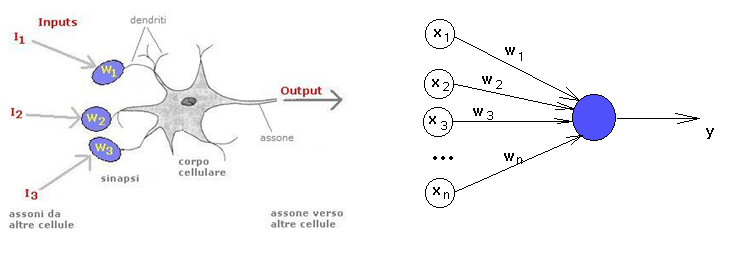
\includegraphics[width=1.0\textwidth]{\teoria/NeuronePitts.png}
 \caption{Modello di calcolo di un neurone (a sinistra) e schema del neurone artificiale (a destra)}
 \label{fig:neuron}
\end{figure}
Si tratta di un'unità di calcolo a N ingressi e 1 uscita. Come si può vedere dall'immagine a
sinistra gli ingressi rappresentano le terminazioni sinaptiche, quindi sono le uscite di altrettanti
neuroni artificiali. A ogni ingresso corrisponde un peso sinaptico $w$, che stabilisce quanto quel
collegamento sinaptico influisca sull'uscita del neurone. Si determina quindi il potenziale del neurone facendo una somma degli ingressi, pesata secondo i pesi $w$. \\
A questa viene applicata una funziona di trasferimento non lineare: 
\begin{equation}
 f(x) = H(\sum_{i}(w_i x_i))
\end{equation} 
ove $H$ è la funzione gradino di Heaviside \parencite{WHeaviside}. Vi sono, come vedremo, diverse altre funzioni non lineari tipicamente utilizzate come funzioni di attivazioni dei neuroni. 
Nel '58 Rosenblatt propone il modello di \emph{Percettrone} rifinendo il modello di neurone a soglia, aggiungendo un termine di \emph{bias} e un algoritmo di apprendimento basato sulla minimizzazione dell'errore, cosiddetto \emph{error back-propagation} \parencite{WPercettrone}.
\begin{equation}
 f(x) = H(\sum_{i}(w_i x_i)+b),\quad ove \quad b = bias \\
\end{equation}
\begin{equation} 
 w_i(t+1) = w_i(t)+\eta \delta x_i(t)
\end{equation}
dove $\eta$ è una costante di apprendimento strettamente positiva che regola la velocità di apprendimento, detta \emph{learning rate} e $\delta$ è la discrepanza tra l'output desiderato e l'effettivo output della rete. 
\\
Il percettrone però era in grado di imparare solo funzioni linearmente separabili. Una maniera per oltrepassare questo limite è di combinare insieme le risposte di più percettroni, secondo architetture multistrato. 
%--------------------------------------------------------------------%--------------------
%	SECTION 2
%--------------------
%--------------------------------------------------------------------

\section{Multi-layer Perceptron}
\label{sec:mlp}
Il Multi-layer Perceptron (\textit{MLP}) o percettrone multi-strato è un tipo di rete feed-forward che mappa un set di input ad un set di output. È la naturale estensione del percettrone singolo e permette di distinguere dati non linearmente separabili.




Il \emph{mlp} possiede le seguenti caratteristiche: 
\begin{itemize}
\item Ogni neurone è un percettrone come quello descritto nella sezione \ref{sec:intro}. Ogni unità possiede quindi una propria funzione d'attivazione non lineare.
\item A ogni connessione tra due neuroni corrisponde un peso sinaptico $w$.
\item È formato da 3 o più strati. In \ref{fig:multilayer} è mostrato un MLP con uno strato di input, un solo strato nascosto (o \emph{hidden layer}) ed uno di output.
\item L'uscita di ogni neurone dello strato precedente è l'ingresso per ogni neurone dello
strato successivo. È quindi una rete \emph{completamente connessa}. Tuttavia, si possono
disconnettere selettivamente settando il peso sinaptico $w$ a 0.
\item La dimensione dell'input e la dimensione dell'output dipendono dal numero di
neuroni di questi due strati. Il numero di neuroni dello strato nascosto è invece
indipendente, anche se influenza di molto le capacità di apprendimento della rete. 
\end{itemize}
%non linearità 
Se ogni neurone utilizzasse una funzione lineare allora si potrebbe ridurre l'intera rete ad una composizione di funzioni lineari. Per questo - come detto prima - ogni neurone possiede una funzione di attivazione non lineare. 

%black box
\subsection{Strati Nascosti}
I cosiddetti \emph{hidden layers} sono una parte molto interessante della rete. Per il teorema di
approssimazione universale \parencite{WApprox}, una rete con un singolo strato nascosto e un numero finiti di
neuroni, può essere addestrata per approssimare una qualsiasi funzione continua su uno spazio compatto di $\mathbb{R}^n$. In altre parole, un singolo strato nascosto è abbastanza potente da imparare un ampio numero di funzioni. Precisamente, una rete a 3 strati è in grado di separare regioni convesse con un numero di lati $\leqslant$ numero neuroni nascosti. 

Reti con un numero di strati nascosti maggiore di 3 vengono chiamate reti neurali profonde o \emph{deep neural network}; esse sono in grado di separare regioni qualsiasi, quindi di approssimare praticamente qualsiasi funzione. Il primo e l’ultimo strato devono avere un numero di neuroni pari alla dimensione dello spazio di ingresso e quello di uscita. Queste sono le terminazioni della \emph{"black box"} che rappresenta la funzione che vogliamo approssimare. 

L'aggiunta di ulteriori strati non cambia \emph{formalmente} il numero di funzioni che si possono approssimare; tuttavia vedremo che nella pratica un numero elevato di strati migliora di gran lunga le performance della rete su determinati task, essendo gli hidden layers gli strati dove la rete memorizza la propria rappresentazione astratta dei dati in ingresso. Nel capitolo 4 vedremo un'architettura all'avanguardia con addirittura 152 strati.
 
%--------------------------------------------------------------------%--------------------
%	SECTION 3
%--------------------
%--------------------------------------------------------------------

\section{Caso di studio: prevedere il profitto di un ristorante}
%%%  30 Coperti - 11 Mesi all'anno
%%%  20 coperti - 38-42 ore di apertura a settimana 
%%%  Profitto in % = Ricavo - Spesa, According to the Restaurant Resource Group, average profit margins for restaurants range from 2 to 6 percent. 
%%% 
Prendendo spunto dalla traccia d'esame di Sistemi Intelligenti M del 2 Aprile 2009:
\begin{quote}
\textit{"Loris è figlio della titolare di una famoso spaccio di piadine nel Riminese e sta tornando in Italia
dopo aver frequentato con successo un prestigioso Master in Business Administration ad Harvard, a
cui si è iscritto inseguendo il sogno di esportare in tutto il mondo la piadina romagnola. Nel lungo
viaggio in prima classe, medita su come presentare alla mamma, che sa essere un tantino restia alle
innovazioni, il progetto di aprire un ristorantino a New York City."}
\end{quote}
Loris ha esportato con successo la piadina a NY, (si veda \parencite{WGradisca}) ma col passare degli anni ha notato alcuni problemi e vuole utilizzare di nuovo le sue brillanti capacità analitiche per migliorare il profitto del suo ambizioso ristorante. \\
I problemi sono 2: 
\begin{enumerate}
\item il ristorante è conosciuto ormai - si sa che tutti vogliono mangiare italiano - ma il numero dei coperti è rimasto a 22, come quelli iniziali; 
\item gli orari di apertura sono troppo lunghi e vi sono alcune zone morte dove il costo di mantenere aperto il ristorante è maggiore rispetto al ricavo dei pochi clienti che si siedono a mangiare durante quelle ore; 
\end{enumerate}
Secondo la National Restaurant Association \parencite{WProfit} \parencite{WRRG}, il profitto medio lordo annuo di un ristorante negli Stati Uniti varia dal 2 al 6\%. Così Loris ha collezionato alcuni dati riguardo agli ultimi anni e - attratto da tutta quest'entusiasmo attorno alle reti neurali - decide di provare ad utilizzarle per trovare il trade-off ottimale di coperti e di orari di apertura settimanali per massimizzare il profitto del suo ristorante. 
\\

Dati questi presupposti, si vedrà nel capitolo \ref{Capitolo2} come implementare da zero un multi-layer perceptron e addestrarlo per suddetto scopo.

\begin{figure}[h!]
 \centering
 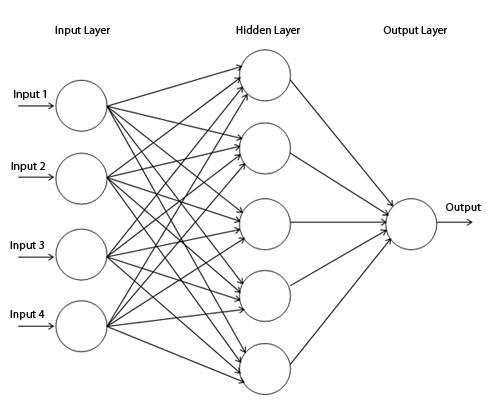
\includegraphics[width=1.0\textwidth]{\teoria/multilayer.png}
 \caption{Struttura di un percettrone multistrato con un solo strato nascosto}
 \label{fig:multilayer}
\end{figure}


% Chapter Template

\chapter{State of the art} % Main chapter title
\label{Chapter2}
\def \teoria {Figures/teoria}
\def \path	 {Figures/C2}

In recent years tremendous progresses have been made with regard to CNN model compression and acceleration. In this chapter an overview of the most significant techniques is provided. Note that details and terminology of CNNs are later explained in chapter 3. 

%--------------------------------------------------------------------%	SECTION 1
%--------------------------------------------------------------------
\section{Model Design vs. Model Compression}
Convolutional neural networks compression can be addressed in two main different ways: the first one is to focus on exploring the best practices to build smaller networks without sacrificing accuracy; the other one consists of taking a pre-trained successful model and compress the existent weights to extract a thinner version of it but with same knowledge, and so the accuracy. \\
This is the first point to keep in mind. 
\newline 
The other distinction is based on which layers to address, namely convolution layers and fully-connected one (layers detailed explanation will follow in chapter 3). This depends on which, among the following, is the priority: 
    \begin{itemize}
        \item  \textbf{acceleration}: most of the computation in CNNs are done in the first convolutional layers; thus these need to be compressed in order to achieve a significant speedup; 
        
        \item \textbf{compression}: most of the parameters are in the last fully connected layers; therefore a reduction on the former is required to save on memory consumption.
    \end{itemize}
    
For the reasons above, each of the presented schemes will be labeled with the possible area of application. 

\newline 
The approaches proposed so far can be classified into four main categories: \emph{(i)} parameter pruning; \emph{(ii)} low-rank factorization; \emph{(iii)} knowledge distillation; \emph{(iv)} compact network design.

%--------------------------------------------------------------------
%	SECTION 2
%--------------------------------------------------------------------

\section{Parameter pruning and sharing}
Pruning was proposed before deep learning became popular, and it has been widely studied in recent years \parencite{brain-damage}. Based on the assumption that lots of parameters in deep networks are unimportant or unnecessary, pruning methods try to remove parameters that are not crucial to the model performance. 
\newline 

In this way, networks becomes more sparse and thus show few benefits: the sparsity of the structure acts as a regularization technique against over-fitting, hence improving the model generalization; the computations involved in the pruned parameters are omitted, thus the computational complexity can be reduced; finally, sparse parameters require less disk storage since they can be stored in compressed formats. 
\newline 

Pruning methods can be applied on both model design and compression and since they address single weights, can be applied on both fully connected and convolution layers. Moreover, they can be further classified into three categories: network pruning, model quantization and structural matrix design.  

\subsection{Network Pruning}
\label{subsec:pruning}
As aforementioned, the core assumption of pruning is that many parameters are redundant and unnecessary. However, techniques differ on how to assess which parameters are less important than others and the granularity of the actual pruning. 

Figure \ref{fig:pruning} shows the various pruning levels for a convolutional layer.

\begin{figure}[h!]
 \centering
 \includegraphics[width=1.0\textwidth]{\path/pruning.jpg} 
 \caption{Different pruning granularity for a $3 \times 3 \times 3$ convolutional filter. Image from \parencite{survey2018}}
 \label{fig:pruning}
\end{figure}

\newline 

\paragraph{Fine-grained pruning}
Fine-grained pruning methods remove parameters in an unstructured way, i.e., any unimportant parameters in the convolutional kernels can be pruned without particular constraint. This gives large degrees of freedom but requires more manual parameter tuning. 

An early approach to network pruning was the biased weight decay \parencite{pruning-biased} that consisted in cutting away weights in a magnitude-based fashion. Later works, as the Optimal Brain Damage \parencite{brain-damage} and the Optimal Brain Surgeon\parencite{brain-surgeon}, assessed the search of unimportant parameters based on the Hessian of the loss function and show better results. 
\\
However, it is unaffordable for deep networks to compute the second order derivatives for each weight due to a huge computational complexity.  

A recent improvement that enabled to prune uninformative weights in a pre-trained CNN model, was proposed by Han et al. in \parencite{deep-compression}. Their \emph{"deep compression framework} consists of three important steps: 
    \begin{enumerate}
        \item pruning redundant connections and retrained the sparse connections; 
        
        \item quantization of the remaining weights;
        
        \item Huffman coding to encode the quantized weights in a loss-less format.  
    \end{enumerate}

By using the former method, Han et. al managed to compress AlexNet\parancite{alexnet} by 35$\times$ with no drop in accuracy; this method achieved state-of-the-art  The pipeline of the former is shown in figure \ref{fig:huffman}


\begin{figure}[h!]
 \centering
 \includegraphics[width=1.0\textwidth]{\path/huffman.jpg} 
 \caption{The three steps compression method proposed in \parencite{deep-compression}: pruning, quantization and encoding.}
 \label{fig:huffman}
\end{figure}

\paragraph{Group-level pruning}
Group-level pruning apply the same sparse pattern on the filters, so that convolutional filters can be represented as thinned dense matrix. An example of this can be seen in figure \ref{fig:group-pruning}.

\begin{figure}[h!]
 \centering
 \includegraphics[width=0.7\textwidth]{\path/group-level.png} 
 \caption{An example of group-level pruning, from  \parencite{survey2018}.}
 \label{fig:group-pruning}
\end{figure}

Since this type of pruning produces thin dense matrices, convolution operation can be implemented as thinned dense matrix multiplication leveraging on the Basic Linear Algebra Subprograms (BLAS) and hence achieving higher speed-ups (almost linear with the sparsity level). 

One way to implement this, is by employing group-sparisity regularizers. As explained in chapter 3, regularizers are added to the loss function in order to penalize too complex models. By applying a group-sparsity regularizer, Lebedev and Lempitsky \parencite{lebedev2} showed how to train a CNN easily with group-sparsified weights. 


\paragraph{Filter-level pruning}
Filter-level pruning, as the name suggests, prunes the individual filters (or channels) of the CNN, thus making the network thinner. After pruning filters on one layer, the following layers' channels are also pruned. For this reason, compared to other pruning, this method is more suited to accelerate deep networks 
\newline 

In order to properly choose the filter channels to prune, custom parameters have to be imposed. For example, it's possible to guide a layer filter pruning by using the next layer's feature map as a guide i.e., by minimizing the reconstruction error on the latter. In this way, the layer will optimize a subset of its filters to obtain the same result as the original model. This strategy has been proposed by \parencite{Luo2017}. 
\newline

Other methods have always applied similar per-layer constraints. 


\paragraph{Considerations}
\begin{itemize}
    \item \textbf{Application}: convolutional and fully-connected 
    
    \item \textbf{Drawbacks}: Pruning techniques are elastic and be applied on every layer and model. However, all pruning criteria require a careful manual setup of sensitivity per-layer, which demands fine-tuning of the new imposed parameters. This can be inconvenient in some scenario. 
\end{itemize}


\subsection{Quantization and Binarization}
Network quantization involves compressing the original network by reducing the number of bits required to represent each weights. This strategy is further classifiable into two groups: \emph{scalar and vector} quantization and \emph{fixed-point} quantization. 

\paragraph{Scalar and vector quantization}
Scalar and vector quantization technique has a long history, and it was original used for data compression. Through this method the original data can be represented by two basic elements: 
 \begin{itemize}
     \item \emph{a codebook} that contains a set of "quantization centers";
     
     \item \emph{a set of quantization codes} used to indicate the assignment of the quantization centers.
 \end{itemize}
 
 Most of the time, the cardinality of quantization centers is far smaller than the number of original parameters. 
 \\
 In addition, the quantization codes can be encoded by lossless encoding methods as Huffman coding, which was also a fundamental gear of the deep compression pipeline mentioned in section \ref{subsec:pruning}. For this reason scalar and vector quantization can achieve high compression ratio and can be applied on both convolutional \parencite{WU2016} and fully-connected layer \parencite{gong}. 

\paragraph{Fixed-point quantization}
Resource consumption of CNN is not only based on the rough number of weights, but also on the activations and the gradient computation during the backward pass in the training phase. To tackle this, fixed-point quantization methods are divided into:
\begin{enumerate}
    \item quantization of weights; 
    
    \item quantization of activations; 
    
    \item quantization of the gradient: these methods are also able to speed-up training, for obvious reasons. 
\end{enumerate}

Compression with 8-16-32 bits fixed-point have been experimented with fair results. [CIT NEEDED]. Interestingly, it has been proposed that 16-bit fixed-point was adequate to train small models, while 32-bit fixed-point were required in the case of bigger nets.  


In the extreme scenario of 1-bit representation of each weight, that is, \emph{binary weight neural networks}, there are also many works that directly train CNNs with binary weights, for instance, BinaryConnect \parencite{binaryconnect}, BinaryNet \parencite{binarynet} and XNOR-Networks \parencite{XNOR}. 

The main idea is to directly learn binary weights or activations during the model training, so that it is possible to get rid of floating computations once for all. 
\newline 

Among all, XNOR-net achieved remarkable results on the ImageNet dataset, outperforming other quantized nets by a large margin. It reached the same accuracy of AlexNet, while saving 32$\times$ memory usage and 58$\times$ faster convolution operations. An overview of XNOR-net is reported in figure \ref{fig:xnor}

\begin{figure}[h!]
 \centering
 \includegraphics[width=1.0\textwidth]{\path/xnor.jpg} 
 \caption{XNOR-Net overview with computation speedups and memory savings. }
 \label{fig:xnor}
\end{figure}

An interesting point made by XNOR-net is that it is the first state-of-the-art network that can be trained on CPUs and can be a candidate for real-time operations. It is indeed already been deployed on smartphone by \parencite{Wxnor-ai}.


\paragraph{Considerations}
\begin{itemize}
    \item \textbf{Application}: convolutional and fully-connected 
    
    \item \textbf{Drawbacks} the accuracy of said binary nets is significantly lowered when dealing with large CNNs such as GoogLeNet. Besides, the approximation techniques for binary weights don't yet take into account the effects on accuracy loss
\end{itemize}
. 

%--------------------------------------------------------------------
%	SECTION 3
%--------------------------------------------------------------------

\newpage
\section{Knowledge Distillation}
Knowledge distillation is different from other methods since it tries to built a smaller model that can have a totally different architecture but same accuracy on the same problem domain. 
\\
Its mechanism resembles much more what happens in the human world: in fact, it works by transferring the knowledge from a large network, \emph{the teacher}, to a much smaller one i.e., \emph{the student}. Hence, it is also called teacher-student network. 

Originally introduced by Caruana et al. \parencite{caruana} only on shallow models, it has been now reproposed. By utilizing what is known as the \emph{"dark knowledge"} transferred from the teacher network, the smaller model can achieve higher accuracy than training merely by the "raw" class labels.

As of 2018, three main works have paved the road to this interesting application: 
\begin{enumerate}
    \item Hinton et. al \parencite{hinton-KD} proposed to improve the student network training with the \emph{softmax} layer's output of the teacher, i.e. the (log)probabilities of each class. This scheme is reported in figure \ref{fig:KD}.
    
    \item Following this line, Romero et al. \parencite{romero-KD} proposed \textit{FitNets} as teachers for thinner and deeper networks. They went further by training the student not only on the softmax probabilities of the teacher but also on its intermediate feature maps.
    
    \item Finally, in \parencite{greci-KD} Zagorukyo and Komodakis proposed an even more interesting approach: the student network was trained on the \emph{attention maps}. Attention  maps are defined as those feature maps where the network held most of its knowledge. Once these maps are found, we can transfer only their content to the student, resulting in an even thinner model. This new branch goes with the name of \emph{Attention Transfer} (AT).
\end{enumerate}

Moreover, the teacher can be an ensemble of models \parencite{Wensemble} with modules called "specialists" who focus on only training the student on sub-parts of the problem. 
Noticeably, these methods did not show the need for regularization techniques such as dropout (see Chapter \ref{Chapter3}) since the transferred knowledge, in a sense, is already filtered and optimized. 


\begin{figure}[h!]
 \centering
 \includegraphics[width=0.7\textwidth]{\path/KD.png} 
 \caption{Teacher-student scheme: the student learn on a mix of }
 \label{fig:KD}
\end{figure}


\paragraph{Considerations}
\begin{itemize}
    \item \textbf{Application}: training from scratch only.
    
    \item \textbf{Drawbacks}: 
Training with KD technique is way less costly. However, currently these approaches can only be applied to classification tasks with softmax loss functions. Another drawback is that certain assumptions are too strong to make the performance comparable to other methods.
\end{itemize}




%--------------------------------------------------------------------
%	SECTION 4
%--------------------------------------------------------------------
\section{Compact Network Design}
While other methods try to optimize execution and memory consumption for a given model without changing its architecture, compact network design aims at designing better models in the first place. 
\\
It is based on some empirical principles that come out over the years, through different breakthroughs in the field. A summary of the former is listed here, while an comprehensive explanation is provided in Chapter 3, where CNN architecture is discussed. 
\\
\\
The elements of an optimal CNN design are:
\begin{itemize}
    \item \emph{micro-architecture design of the network building blocks}
    
    \item \emph{$[1 \times 1]$ convolutions}
    
    \item \emph{network branching}
    
    \item \emph{depthwise separable convolution}
    
\end{itemize}



\paragraph{Considerations}
\begin{itemize}
    \item \textbf{Application}: training from scratch, most of the time. However, these principles can be combined with low-rank approximations methods when substituing a layer with a new approximated block, that could follow these rules. 
    
    \item \textbf{Drawbacks}: Since this method only aims at building better models, it does not make much sense to compare it to the others in terms of advantages and pifalls. It is just a general framework of good practices to be kept in mind
\end{itemize}


%--------------------------------------------------------------------
%	SECTION 5
%--------------------------------------------------------------------
\section{Low-rank Factorization}
The convolutional kernel of a convolution layer $W \in R^{s \times t \times d \times d}$ is a 4-D tensor, with the four dimension corresponding to the number of input and output channels and the kernel size respectively (here squared for simplicity). Low rank factorization methods try to find a way to determine an approximate tensor $\hat{W}$ that is close to $W$ but has far less parameters, facilitating the computations. 
\newline 

This can be done in a variety of ways that all plays on how many layers we want to arrange the decomposed tensor $\hat{W}$. For instance, it can be arranged in 2 layers holding 2 dimensions of the original one, or in 4 by one, or even in asymettric 3 layers decomposition. The former is possible by manipulating the tensor and utilizing different decomposition techniques, such as SVD \citep{zhang2015SVD}, Tucker \citep{Tucker-mobile}, CPD \citep{lebedev} and others.
\newline

This approach can be embeddable in a decomposition pipeline as: 
\begin{itemize}
  \item select an over-parametrized layer; 
  
  \item compress the layer with one of the mentioned algorithms; 
  
  \item embed the decomposed layer into the model instead of the old one; 
  
  \item perform some iteration of fine-tuning to recover the approximation error; 
  
  \item start again. 
\end{itemize}

As these methods will be seen in details in chapter \ref{Chapter4}, we can omit, for the moment, the details. 


\paragraph{Considerations}
\begin{itemize}
    \item \textbf{Application}: pre-trained models and new architectures, both FC and convolutional layers. 
    
    \item \textbf{Drawbacks}: As we will see, these methods are good candidates to be implemented in a pipeline, i.e. their integration is straightforward. However, tensor decomposition algorithms are expensive and not so easy to play around at first. Besides, the compression happens layer by layer and therefore does not take into account the loss of information related to another layer. Furthermore, training could take many iterations before convergence. 
\end{itemize}

%--------------------------------------------------------------------
%	SECTION 6
%--------------------------------------------------------------------
\section{Other methods}
There are several other methods to address this new trend like \emph{transferred convolutional filters}, \emph{dynamic capacity networks}, etc. For an exhaustive reference lists, please refer to \parencite{survey2017}. 

Remarkable trends are also showing up on the hardware side of the challenge, with FPGA/ASIC-based accelerators re-gaining popularity over GPUs, aiming at real-time applications, low energy consumption and high-throughput optimization 

This is important for the scope of this thesis, as the final goal of this project is to deploy optimized models on FPGA, Intel Movidius or Raspberry Pi. 

%--------------------------------------------------------------------
%	SECTION 7
%--------------------------------------------------------------------
\section{Discussion}
The presented methods are orthogonal. It is possible to combine two or three of them together to maximize the compression by applying the best suited technique on a specific scenario. For example, in the case of object detection where both convolution and fully connected layers are needed, it is feasible to compress the former with low-rank factorization and the latter with pruning. 
Moreover, when a small accuracy drop is tolerable, quantization can also be applied as a final step after the aforementioned methods. 
\newline 

One pitfall, however, is that most of these methods require non trivial hyper-parameters configurations. Hence, it is not straightforward to combine them as one could get stuck in the hyper-parameters tuning loop before finding the best setup. This is probably due to the early age of these techniques. 
\newline 

As for this work, since the future goal will be to optimize custom pre-trained models of the VisionLab of the University of Bologna, only two methods are feasible candidates: network pruning and low-rank factorization. Among these, the latter is the only one that provides a possible end-to-end pipeline to the problem. 
\newline 

Therefore, this thesis will focus on the low-rank factorization technique; specifically, on further developing \emph{tensor decomposition methods}, which do not seem to be fully explored yet and could have promising applications.  
% Chapter Template

\chapter{Reti Neurali Convoluzionali} % Main chapter title
\label{Capitolo3}
\def \teoria {Figures/teoria}
\def \path	 {Figures/C3}
%--------------------------------------------------------------------%	SECTION 1
%--------------------------------------------------------------------
%% da completare
In questo capitolo si introduce una panoramica generale sulle reti neurali convoluzionali. Essendo un argomento vasto, una trattazione teorica approfondita sarebbe materia di una tesi di laurea, ragion per cui gli argomenti sono introdotti con lo scopo di avere un'infarinatura per comprendere le applicazioni sviluppate nei capitoli successivi. 
\section{Breve introduzione}
La reti neurali convoluzionali, alle quali ci riferiremo con l'abbrevazione \emph{CNN} - dall'inglese \emph{Convolutional Neural Network}, sono un'evoluzione delle normali reti artificiali profonde caratterizzate da una particolare architettura estremamente vantaggiosa per compiti visivi (e non), che le ha rese negli anni molto efficaci e popolari. Sono state ispirate dalle ricerche biologiche di Hubel e Wiesel i quali, studiando il cervello dei gatti, avevano scoperto che la loro corteccia visiva conteneva una complessa struttura di cellule. Quest'ultime erano sensibili a piccole parti locali del campo visivo, detti campi recettivi \emph{(receptive fields)}. Agivano quindi da filtri locali perfetti per comprendere la correlazione locale degli oggetti in un'immagine. Essendo questi sistemi i più efficienti in natura per la comprensione delle immagini, i ricercatori hanno tentato di simularli. 

%--------------------------------------------------------------------
%	SECTION 2
%--------------------------------------------------------------------

\section{Architettura}
Le CNN sono reti neurali profonde costituite da diversi strati che fungono da estrattori delle features ed una rete completamente connessa alla fine, che funge da classificatore, come raffigurato in figura \ref{fig:cnn1}. \\
\begin{figure}[h!]
 \centering
 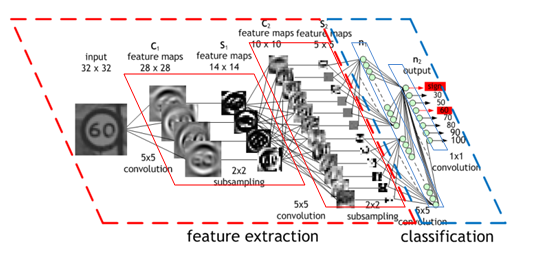
\includegraphics[width=1.0\textwidth]{\path/CNN-expl.png} 
 \caption{Architettura di una CNN che classifica segnali stradali: si evidenzia la divisione tra gli strati che fungono da feature extractor ed il classificatore finale}
 \label{fig:cnn1}
\end{figure}
Questi strati in cui si estraggono le caratteristiche delle immagini sono detti strati di convoluzione, e sono generalmente seguiti da una funzione non lineare e un passo di \emph{pooling}. Vi possono poi essere degli strati di elaborazione dell'immagine, come quello di normalizzazione del contrasto, si veda \fig{ref:cnn2}.
\begin{figure}[h!]
 \centering
 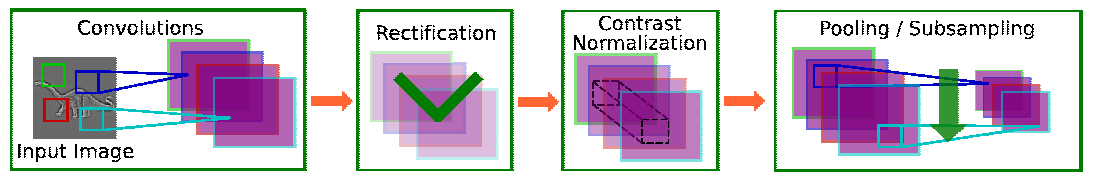
\includegraphics[width=1.0\textwidth]{\path/CNN-features.png} 
 \caption{I diversi strati tipici di una CNN}
 \label{fig:cnn2}
\end{figure}
Convoluzione e pooling hanno come scopo quello di estrarre le caratteristiche, mentre l’unità non lineare serve a rafforzare le caratteristiche più forti e indebolire quelle meno importanti, ovvero quelle che hanno stimolato meno i neuroni (si dice che fa da “squashing”). \\
Sempre dalla figura \ref{fig:cnn1}, possiamo inoltre notare che, per ogni immagine in input, corrispondono nei vari strati, diversi gruppi di immagini, che vengono chiamate \emph{feature maps}. Le feature maps sono il risultato dell'operazione di convoluzione svolta tramite un banco di filtri, chiamati anche kernel, che altro non sono che delle matrici con dei valori utili a ricercare determinate caratteristiche nelle immagini.\\
Infine, terminati i convolutional layers, le feature maps vengono “srotolate” in vettori e affidate ad una rete neurale "classica" che esegue la classificazione finale. 

Il numero di strati di convoluzione è arbitrario. Inizialmente, quando le CNN divennero famose grazie a Y.LeCun, che addestrò una CNN chiamata \emph{"LeNet5"} al riconoscimento dei numeri \parencite{lenet}, questo numero era compreso tra 2-5. Nel 2012, Alex Krizhevsky et al \parencite{imagenet2012} addestrarono una rete costituita da 5 strati di convoluzione, 60 milioni di parametri e 650 mila neuroni. Ottennero la migliore percentuale d'errore al mondo sul dataset ImageNet ILSVRC-2010, contenente 1,2 milioni di immagini divise in 1000 categorie. \\
Da allora le cose si sono evolute con una velocità disaramente, e l'ImageNet challenge del 2015, è stata vinta da una rete con 152 strati \parencite{resnet}. Nel capitolo \ref{Capitolo5} si farà un confronto tra quest'ultima rete, soprannominata \emph{"ResNet"} e la capostipite LeNet5 su un task di classificazione.   
\subsection{Strato di Convoluzione}
Per comprendere appieno quello che avviene in una CNN, occorre introdurre il concetto di convoluzione fra matrici, e capire come questo sia importante per applicare dei filtri ad un'immagine digitale.
\\
Un’immagine digitale può essere considerata come una matrice A di dimensione MxN valori reali o discreti. Ogni valore della matrice prende il nome di pixel e i suoi indici sono anche chiamati coordinate: ogni pixel $A(m,n)$ rappresenta l’intensità nella posizione indicata dagli indici. \\ 
Si definisce “filtro” o “kernel” una trasformazione applicata ad un’immagine. Come detto prima, questi filtri sono a loro volta della matrici; la trasformazione quindi si effettua appunto tramite un'operazione di convoluzione tra l'immagine in ingresso ed il filtro.
La convoluzione, discreta nel caso di immagini digitali, si può definire come: 
%% INSERIRE EQUZIONEI %%% 
$$
y[m,n] = x[m,n] \circledast h[m,n] = \sum^{m}\sum^{n}x[i,j]\times h[m-i,n-j]
$$
Ogni pixel di $y[m,n]$ è così il risultato di una somma pesata tramite $h[m,n]$ della sottoregione che ha centro nel pixel indicato dalle coordinate m,n. Un esempio di convoluzione è rappresentato in figura \ref{fig:convolution}. 
\begin{figure}[h!]
 \centering
 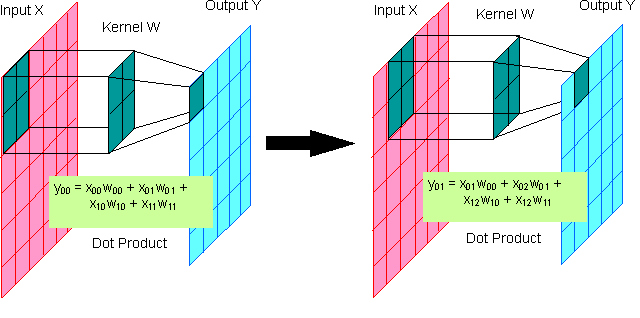
\includegraphics[width=0.7\textwidth]{\path/convolution.png} 
 \caption{Convoluzione con un kernel: primi due step}
 \label{fig:convolution}
\end{figure}
\\
Nei convolutional layers viene quindi fatta un'operazione di convoluzione tra l'immagine/i in ingresso
e un numero arbitrario K di filtri. Questi filtri hanno valori tali da ottenere in uscita un riconoscimento di determinate caratteristiche. \\
I valori dei filtri sono all'inizio scelti casualmente, e vengono poi migliorati ad ogni iterazione mediante l'algoritmo di backpropagation, visto nel Capitolo \ref{Capitolo2}. Così facendo la rete addestra i suoi filtri ad estrarre le features più importanti degli esempi del training set; cambiando training set i valori dei
filtri saranno diversi.
Ad esempio, i valori dei filtri di una rete allenata con immagini di pali verticali saranno diversi da quella allenata con immagini di palloni da calcio; nel primo caso i valori saranno calibrati per riconoscere lunghi orientamenti verticali, mentre
nel secondo per riconoscere i confini sferici. 

Nelle reti convoluzionali quindi, l'algoritmo di Backpropagation migliora i valori dei filtri della rete, è lì quindi che si accumula l'apprendimento. I neuroni, in queste reti, devono intendersi come i singoli filtri.\\
\\
Vi sono diversi \emph{hyperparameters} da settare manualmente negli strati di convoluzione: 
\begin{enumerate}
\item la misura del filtro $F$: chiamato anche \emph{receptive field}. Ogni filtro cerca una determinata caratteristica in un'area locale dell'immagine, la sua misura quindi è il campo recettivo del singolo neurone. Tipicamente sono 3x3, 5x5 o 7x7.

\item il numero $K$ di filtri: per ogni strato, questo valore definisce la profondità dell'output dell'operazione di convoluzione. Infatti, mettendo una sopra l'altra le feature maps, si ottiene un cubo in cui ogni "fetta" è il risultato dell'operazione tra l'immagine in ingresso ed il corrispettivo filtro. La profondità di questo cubo dipende appunto dal numero dei filtri. 

\item lo \emph{"Stride"} S: definisce di quanti pixel si muove il filtro della convoluzione ad ogni passo. Se lo stride è settato a 2, il filtro salterà 2 pixel alla volta, producendo quindi un output più piccolo. 

\item il \emph{"padding"} P: definisce la misura con la quale si vuole aggiungere degli "0" all'input per preservare la dimensione in output. In generale, quando lo stride S=1, un valore di  $P = (F - 1)/2$ garantisce che l'output avrà le stesse dimensioni dell'input. 
\end{enumerate}
\\
%% pezzo sulla dimensione in output %% 
Quando si elaborano delle immagini con le CNN si hanno generalmente in ingresso degli input tridimensionali, caratterizzati dall'altezza $H_1$, l'ampiezza $W_1$ e il numero di canali di colore $D_1$. Conoscendo i parametri sopra specificati si può calcolare la dimensione dell'output di un layer di convoluzione: 
\begin{align*}
H_2 = (H_1 - F + 2P)/S + 1\\
W_2 = (H_1 - F + 2P)/S + 1\\
D_2 = K
\end{align*}
%% 
A questo proposito si osservi un esempio di "volume di neuroni" del primo strato di convoluzione in figura \ref{fig:depth}. Ogni neurone è collegato spazialmente solo ad 1 regione locale dell'input ma per tutta la profondità (i.e. i 3 canali del colore). Si noti che ci sono 5 neuroni lungo la profondità e tutti guardano alla stessa regione dell'input.
\begin{figure}[h!]
 \centering
 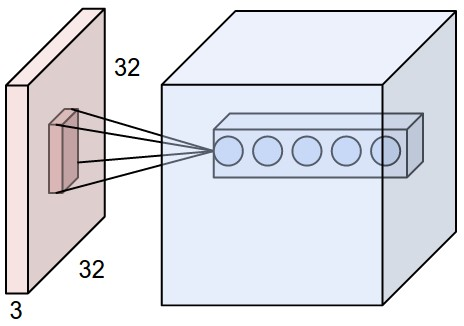
\includegraphics[width=0.4\textwidth]{\path/depthcol.jpeg} 
 \caption{Ogni neurone è connesso a solo 1 regione locale dell'input ma a tutta la profondità (i.e. canali colori). La depth dell'output è data dal numero K di filtri, in questo caso 5}
 \label{fig:depth}
\end{figure}\\
Gli strati di convoluzione mostrano molte proprietà interessanti.
In primo luogo, se l'immagine in input viene traslata, l'output della feature map sarà traslato della stessa quantità ma rimarrà invariato altrove. Questa proprietà è alla base della robustezza rispetto alle traslazioni e alle distorsioni dell'immagine in ingresso; in secondo luogo, mettendo in fila diversi strati di convoluzione si ottiene una rete capace di avere una comprensione più "astratta" dell'immagine in ingresso. Il primo strato di convoluzione si occupa di estrarre features direttamente dai pixel grezzi dell'immagine e li memorizza nelle feature maps. Questo output diviene poi l'input di un successivo livello di convoluzione, il quale andrà a fare una seconda estrazione delle caratteristiche, combinando le informazioni dello strato precedente. Da questa astrazione a più livelli deriva una maggior comprensione delle features. \\
\subsection{Strato di ReLU}
Nel capitolo \ref{Capitolo2} si è detto che la funzione sigmoide non era la più efficiente. Difatti, negli anni si è stabilita con sicurezza la \emph{Rectified Linear Unit} (ReLU) come funzione d'attivazione più efficace. La ReLU è più verosimile alla modalità di attivazione biologica dei nostri neuroni\parencite{Relu}, ed è definita come: 
$$
f(x) = max(0,x)
$$ 
Y. LeCun ha dichiarato che la ReLU è inaspettatamente \emph{“l'elemento
singolo più importante di tutta l'architettura per un sistema di riconoscimento”}. Questo può essere dovuto principalmente a 2 motivi:
\begin{enumerate}
\item la polarità delle caratteristiche è molto spesso irrilevante per riconoscere gli oggetti;
\item la ReLU evita che quando si esegue pooling (sezione \ref{subsec:pooling}) due caratteristiche entrambe importanti ma con polarità opposte si cancellino fra loro
\end{enumerate}
\subsection{Strato di Pooling}
\label{subsec:pooling}
Un'altra proprietà che si vuole ottenere per migliorare i risultati sulla visione artificiale è il riconoscimento delle features indipendentemente dalla posizione nell'immagine, perché
l'obiettivo è quello di rafforzare l'efficacia contro le
traslazioni e le distorsioni. Questo si può ottenere diminuendo la risoluzione spaziale dell'immagine, il che favorisce una maggiore velocità di computazione ed è al contempo una contromisura contro l'overfitting, dato che si diminuisce il numero di parametri.\\ 
Lo strato di pooling ottiene in ingresso N immagini di una risoluzione e restituisce in uscita lo stesso numero di immagini, ma con una risoluzione ridotta in una certa misura, solitamente del $75\%$. Infatti, la forma più comune di pooling layer utilizza dei filtri 2x2, che dividono l'immagine in zone di 4 pixel non sovrapposte e per ogni zona scelgono un solo pixel. \\
\\
I criteri con cui scegliere il pixel vincente sono diversi:
\begin{itemize}
\item average pooling: si calcola il valore medio sui pixel del pool;
\item median pooling: si calcola la mediana dei valori dei pixel del pool;
\item LP-pooling: si calcola la p-norma della matrice dei pixel;
\item max pooling: si sceglie il pixel col valore più alto; 
\end{itemize}
\\
Di questi, quello che si è dimostrato più efficace è il \emph{max pooling}, figura \ref{fig:maxpool}.
\begin{figure}[h!]
 \centering
 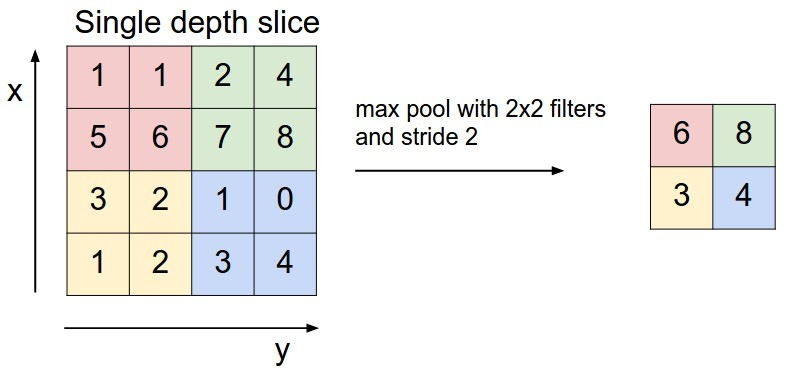
\includegraphics[width=0.8\textwidth]{\path/maxpool.jpeg} 
 \caption{Max pooling: in uscita l'immagine avrà 1/4 dei pixel di partenza.}
 \label{fig:maxpool}
\end{figure}
Attraversando la rete si avrà gradualmente un numero di feature maps  più alto e quindi della ricchezza della rappresentazione delle features; ed una diminuzione della risoluzione dell'input. Questi fattori combinati insieme donano un forte grado di invarianza alle trasformazioni geometriche dell'input.
 
\subsection{Strato completamente connesso (FC)}
%% menzionare che adesso si usa la convoluzione %% 
Nello strato completamente connesso, tutti gli input provenienti dai layer di convoluzione vengono dati in ingresso ad una normale rete neurale completamente connessa che fungerà da classificatore. I calcoli in questa parte finale sono quindi uguali alle moltiplicazioni tra matrici visti nel Capitolo \ref{Capitolo2}. \\
Ultimamente però, si è notato che, eccetto per la modalità di connessione, questi neuroni sono funzionalmente identici a quelli dei layer di convoluzione (entrambi computano moltiplicazioni fra matrici). Quindi si possono sostituire con degli strati di convoluzione che hanno un receptive field di 1x1\parencite{WCS231layer}. 

In figura \ref{fig:cnn4} è rappresentata l'architettura completa di una CNN. Si noti come la risoluzione dell'immagine si riduca ad ogni strato di pooling (chiamato anche subsampling) e come ogni pixel delle feature maps derivi dal campo recettivo sull'insieme di tutte le feature maps del livello precedente. \\
In figura \ref{fig:cnn3} invece, si può osservare una CNN nell'atto di classificazione di un'auto. Sono visualizzati i filtri della rete durante tutti i vari livelli di elaborazionde dell'input, per poi terminare in uno strato completamente connesso che da in output una probabilità. Questa probabilità è poi tradotta in uno score, da cui si sceglie la classe vincente. 
\begin{figure}[h!]
 \centering
 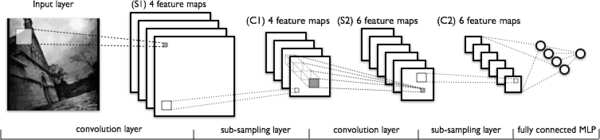
\includegraphics[width=1.0\textwidth]{\path/cnn-architecture.png} 
 \caption{Architettura di una CNN}
 \label{fig:cnn4}
\end{figure}

\begin{figure}[h!]
 \centering
 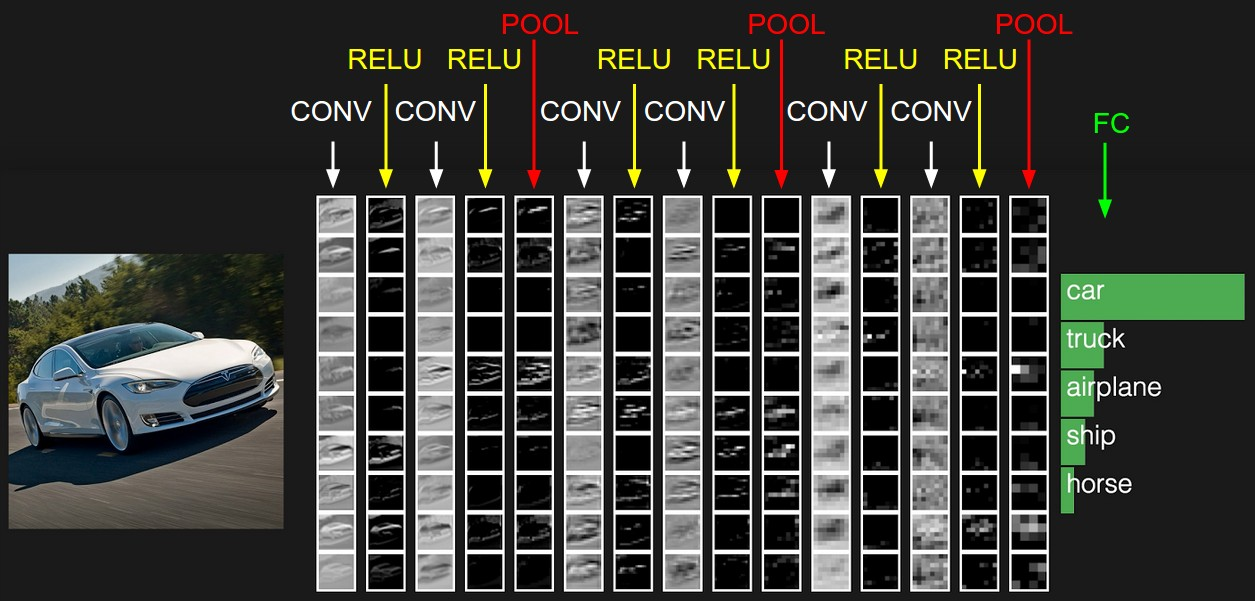
\includegraphics[width=1.0\textwidth]{\path/convnet.jpeg} 
 \caption{Tipica CNN in un task di classificazione; la classe vincente è quella con la probabilità più alta, indicata alla fine}
 \label{fig:cnn3}
\end{figure}
%--------------------------------------------------------------------
%	SECTION 3
%--------------------------------------------------------------------
\section{Applicazioni e risultati}
L'alta efficacia, la peculiare, vantaggiosa architettura insieme con l'enorme progresso tecnologico dell'hardware, hanno reso le CNN il sistema più promettente per compiti di visivo, con i più svariati ambiti applicativi come: riconoscimento e tagging facciale (si pensi a Facebook), ricerca intelligente di immagini (si pensi a Google Photos), automobili autonome, smartphone, robot, droni, (video)giochi ed altro. Le CNN hanno avuto eccellenti risultati anche nell'elaborazione naturale del linguaggio; nella scoperta di farmaci, poiché predicendo le interazioni tra determinate molecole e proteine hanno contribuito a scoprire potenziali biomolecole per il trattamento dell'ebola\parencite{WCNN}, tanto per citarne altri.\\
Già 3 anni fa, in un articolo pubblicato dal dipartimento di visione artificiale del KTH \parencite{Overfeat}, ha utilizzato ”OverFeat”, una CNN pubblica allenata per ILSVRC13, una competizione annuale di riconoscimento degli oggetti. L'articolo sottolinea come abbiano utilizzato questa CNN “off-the-shelf” ovvero già pronta e, senza allenarla ulteriormente, testandola contro altri metodi allo stato dell'arte finemente perfezionati sviluppati fino ad allora. Come test hanno scelto attività gradualmente sempre più lontane dall'originario compito per cui OverFeat è stata addestrata e, con enorme stupore, hanno verificato che OverFeat surclassa i suddetti metodi su qualsiasi dataset (si rimanda all'articolo per i dettagli) nonostante sia stata allenata solo mediante l'ImageNet. L'articolo si chiude con una frase che qui cito:
\begin{quote}
\emph{“Thus, it can be concluded that from now on, deep learning with CNN has to be considered as the primary candidate in essentially any visual recognition task.”}
\end{quote}\\
\subsection{Confronto con l'uomo}
Nel 2011, le CNN hanno la prima volta battuto l’uomo raggiungendo un errore di 0.56\% contro l’1.16\% degli umani sul riconoscimento dei segnali stradali nella competizione “German Traffic Sign competition run by IJCNN 2011”.\\
Un altro compito che è sempre stato difficile per la visione artificiale era il riconoscimento di visi parzialmente occlusi, capovolti o spostati di diverse angolazioni. Tuttavia, nel 2015 un team del Yahoo Labs, è riuscito a far apprendere anche questo compito ad una CNN\parencite{WMit}.

L'ultima pietra migliare in ordine cronologico della sfida "Uomo vs. Macchina" è senza dubbio quella di \textsc{AlphaGo}\parencite{WAlphaGo}. AlphaGo è il primo programma a riuscire a battere un giocatore umano professionista (Lee Sedol, 18 volte campione del mondo) all'antico gioco cinese di Go. \\
Go è conosciuto per essere computazionalmente estremamente complesso: vi sono $10^{170}$ possibili combinazioni della scacchiera, un numero più alto degli atomi dell'Universo conosciuto. È quindi inaffrontabile con un approccio a "forza bruta". 
\\
AlphaGo si basa su una combinazione di deep learning + tree search. In particolare, utilizza 3 CNN: 2 "policy network" per scegliere la strategia più vincente ed 1 "value network" come funzione euristica per valutare la bontà di un'ipotetica mossa. In più, l'output di queste reti è combinato con una "Montecarlo Tree Search" per avere una risposta finale sulla prossima mossa da giocare. Maggiori dettagli si trovano sul lungo paper pubblicato da DeepMind\parencite{AlphaGo}. \\
\\
Questi risultati bastano per comprendere la potenzialità delle convolutional neural networks.

% Chapter Template

\chapter{CNN: implementazione e addestramento} % Main chapter title

\label{Capitolo3} % Change X to a consecutive number; for referencing this chapter elsewhere, use \ref{ChapterX}

%--------------------------------------------------------------------
%	SECTION 1
%--------------------------------------------------------------------

\section{Il framework Torch}





%--------------------------------------------------------------------
%	SECTION 2
%--------------------------------------------------------------------

\section{Modello di CNN basato su LeNet}

\subsection{Strato di Convoluzione}

\subsection{Strato di Pooling}

\subsection{Strato completamente connesso (FC)}


%--------------------------------------------------------------------
%	SECTION 3
%--------------------------------------------------------------------

\section{Dataset d'esempio: CIFAR}

\section{Addestramento su CIFAR}


Vedremo nel capitolo seguente un confronto dei risultati di una CNN con un'archittettura allo stato dell'arte addestrata sullo stesso dataset. 


 
\chapter{Addestrare un modello allo stato dell'arte} % Main chapter title
\label{Capitolo5} % Change X to a consecutive number; for referencing this chapter elsewhere, use \ref{ChapterX}
\def \path {Figures/C5}
%--------------------------------------------------------------------
%	SECTION 1
%--------------------------------------------------------------------
\section{Deep Residual Network}
Menzionata nel Capitolo \ref{Capitolo3} a causa del clamore riscosso per l'incredibilmente bassa percentuale d'errore nella ImageNet Challenge del 2015, la \emph{Deep Residual Network} - o ResNet - è una CNN \emph{molto} profonda presentata da Microsoft Research Asia\parencite{resnet} che ha stravolto tutti i record in classification, detection e localization. 
\\ 
L'architettura è modulare: si basa su un blocco detto \emph{"residual block"} (figura \ref{fig:residual}) che viene ripetuto N volte, prima dell'ultimo strato di classificazione. L'idea dietro a questo blocco viene chiamata \emph{residual learning} e funziona così: 
\begin{enumerate}
\item l'input $x$ va attraverso una serie \texttt{conv-relu-conv} dando in output un certo $F(x)$
\item a questo viene aggiunto l'input originale: $H(x) = F(x) + x$
\end{enumerate}\\ 
$F(x)$ è chiamato residual learning. 
\begin{figure}[h!]
 \centering
 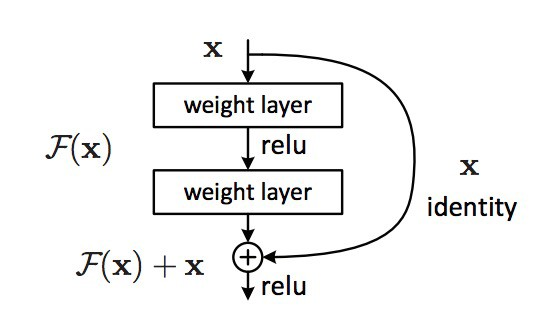
\includegraphics[width=0.6\textwidth]{\path/residual.jpg} 
 \caption{Un "Residual Block", all'input viene aggiunto F(x) che è il residual}
 \label{fig:residual}
\end{figure}

Nelle CNN normalmente si passa direttamente da $x$ a $F(x)$, la quale è una rappresentazione completamente nuova che non mantiene l'informazione dell'input originale. La novità qui, invece, consiste nel mantenere queste informazioni lungo tutta la rete; ogni blocco esegue una sorta di fine-tuning delle informazioni apprese negli strati precedenti, e secondo gli autori è più facile ottimizzare un "residual mapping" anziché un "unreferenced mapping". 
\\
Un esempio della profondità di ResNet è rappresentato in figura \ref{fig:resnet}, dove viene confrontata la versione da 34 strati con la VGG-Network, la rete più profonda che venne presentata 2 anni prima. 

\begin{figure}[h!]
 \centering
 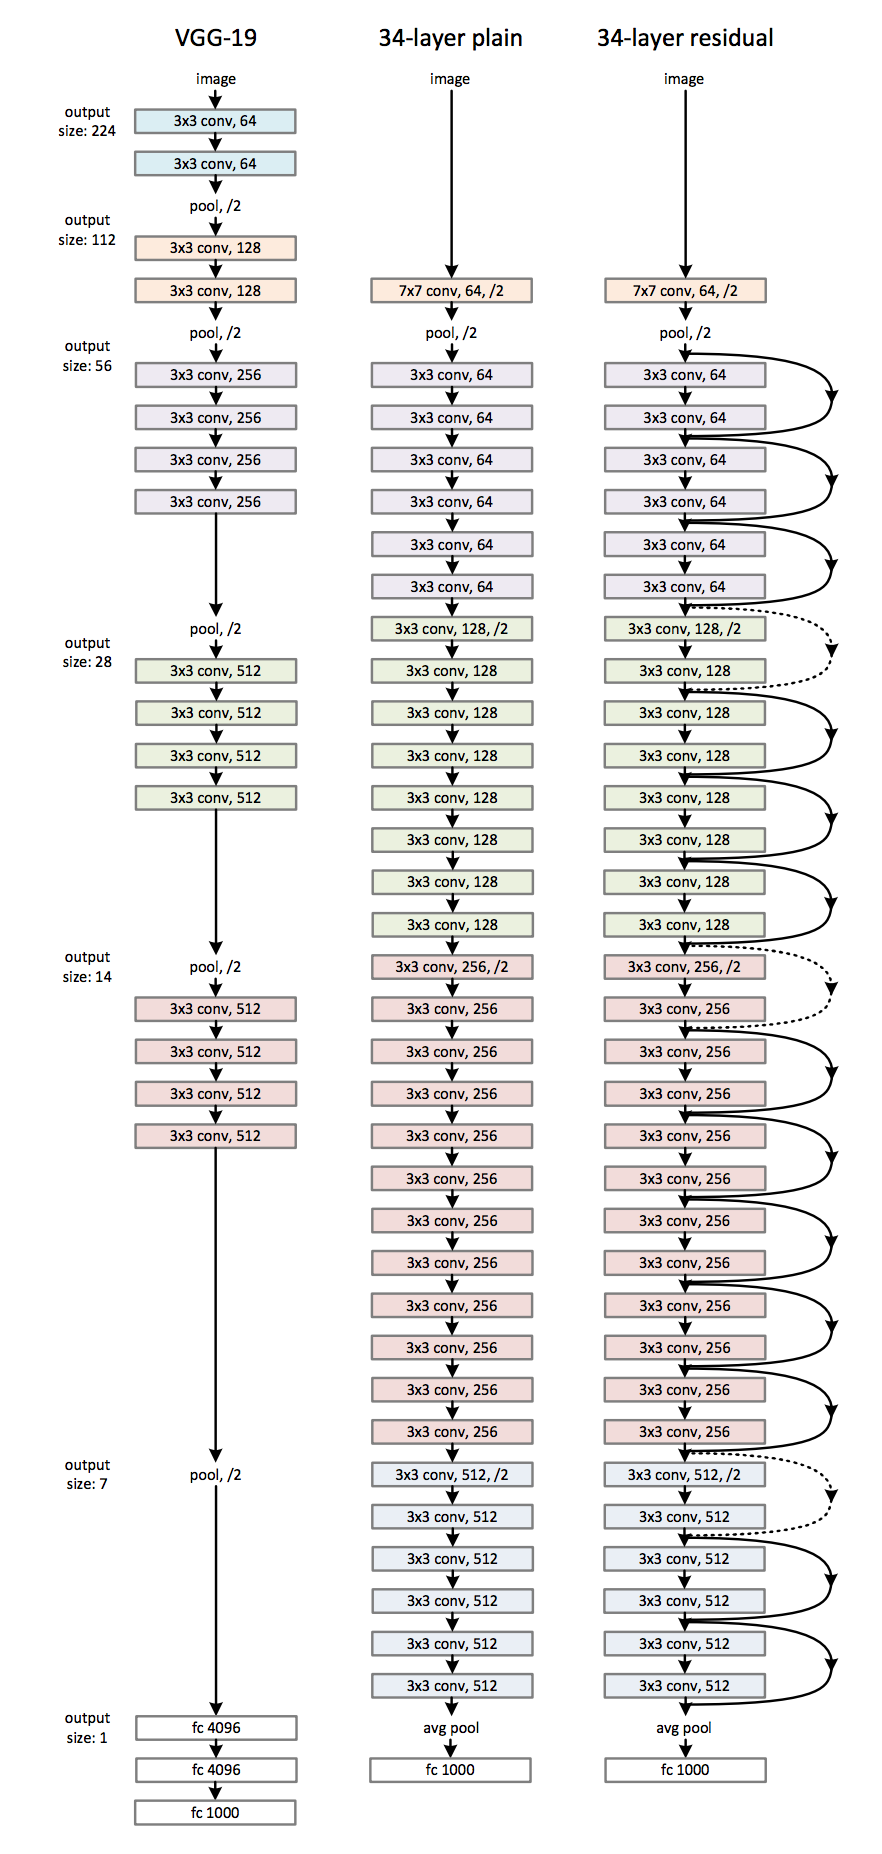
\includegraphics[width=0.7\textwidth]{\path/resnet.png} 
 \caption{Confronto architetture: VGG-Net la più innovativa della competizione ILSVRC 2014, rete classica a 34 strati (centro), Residual Network a 34 strati (sinistra). }
 \label{fig:resnet}
\end{figure}
\\
Un'altra ragione per cui ResNet è stupefacente è che la backpropagation funziona meglio a causa delle somme di ogni layer che distribuiscono la derivata lungo la rete. Inoltre, avere queste scorciatoie che non passano attraverso \texttt{conv-relu} aiuta contro il cruciale problema dei \emph{vanishing gradients}. Quando si usano molti layer uno sull'altro si corre il rischio di non riuscire ad ottimizzare l'apprendimento perché l'errore calcolato con la backprop si perde tra i vari strati e dopo alcuni layer arriva un gradiente nullo che non aiuta nell'apprendimento. Per questa ragione anche, il paper di ResNet è importante: ha dimostrato come poter costruire CNN molto profonde (numero di strati > 100) riuscendo a completare l'apprendimento ed avere inoltre risultati allo stato dell'arte. \\
Tuttavia, altre analisi sul successo di ResNet\parencite{restudy} sostengono il contrario: anche in essa il problema dei vanishing gradients si manifesta dopo \~20 moduli, e quindi la profondità da sola non può essere la caratteristica principale della rete. Suggeriscono invece, che la rete si comporti come un gruppo di "sotto-reti" più piccole che contribuiscono insieme a generare la risposta corretta.\\
È sicuramente un argomento recente e complesso; per ulteriori dettagli si rimanda alla bibliografia. 
 %--------------------------------------------------------------------
%	SECTION 2
%--------------------------------------------------------------------
\section{Implementazione di ResNet di Facebook}
L'implementazione di ResNet è decisamente complessa ma fortunatamente nella community si rilasciano spesso le implementazioni dei modelli più popolari per stimolare i ricercatori a riprodurre gli esperimenti e migliorare sempre di più lo stato dell'arte. A questo proposito Facebook ha rilasciato il codice per diversi modelli di ResNet da 18-34-50-101-152-200 strati. \\
Nei seguenti snippet, vi è l'implementazione della scorciatoia identità e del residual block: 

\begin{lstlisting}[language={[5.2]Lua}]
-- The shortcut layer is either identity or 1x1 convolution
   local function shortcut(nInputPlane, nOutputPlane, stride)
      local useConv = shortcutType == 'C' or
         (shortcutType == 'B' and nInputPlane ~= nOutputPlane)
      if useConv then
         -- 1x1 convolution
         return nn.Sequential()
            :add(Convolution(nInputPlane, nOutputPlane, 1, 1, stride, stride))
            :add(SBatchNorm(nOutputPlane))
      elseif nInputPlane ~= nOutputPlane then
         -- Strided, zero-padded identity shortcut
         return nn.Sequential()
            :add(nn.SpatialAveragePooling(1, 1, stride, stride))
            :add(nn.Concat(2)
               :add(nn.Identity())
               :add(nn.MulConstant(0)))
      else
         return nn.Identity()
      end
   end

   -- The basic residual layer block for 18 and 34 layer network, and the
   -- CIFAR networks
   local function basicblock(n, stride)
      local nInputPlane = iChannels
      iChannels = n

      local s = nn.Sequential()
      s:add(Convolution(nInputPlane,n,3,3,stride,stride,1,1))
      s:add(SBatchNorm(n))
      s:add(ReLU(true))
      s:add(Convolution(n,n,3,3,1,1,1,1))
      s:add(SBatchNorm(n))

      return nn.Sequential()
         :add(nn.ConcatTable()
            :add(s)
            :add(shortcut(nInputPlane, n, stride)))
         :add(nn.CAddTable(true))
         :add(ReLU(true))
   end
\end{lstlisting}
 
Microsoft ha addestrato ResNet per circa 3 settimane su 8 GPU di ultima generazione. Dato l'evidente mancanza di hardware opportuno per un'"impresa" del genera si è deciso di utilizzare il modello più piccolo, quello a 18 strati. In apprendice \ref{AppendixB} è mostrata una rappresentazione testuale del modello, ove se ne può apprezzare la complessità e lunghezza. 


%--------------------------------------------------------------------
%	SECTION 3
%--------------------------------------------------------------------
\section{Addestramento su CIFAR}
Si è addestrato il modello ResNet-18 su CIFAR10 per circa 160 epoche. I risultati sul training e validation set sono presentati rispettivamente in figura e figura. Sull'asse X vi sono le epoch di training, sull'asse Y la percentuale di errore. 
\\
La rete da in uscita le 10 classi più probabili; con top1 s'intende quando la classe corretta è quella in uscita più probabile mentre con top5 quando la classe corretta è tra le prime 5 più probabili. \\
\begin{figure}[h!]
 \centering
 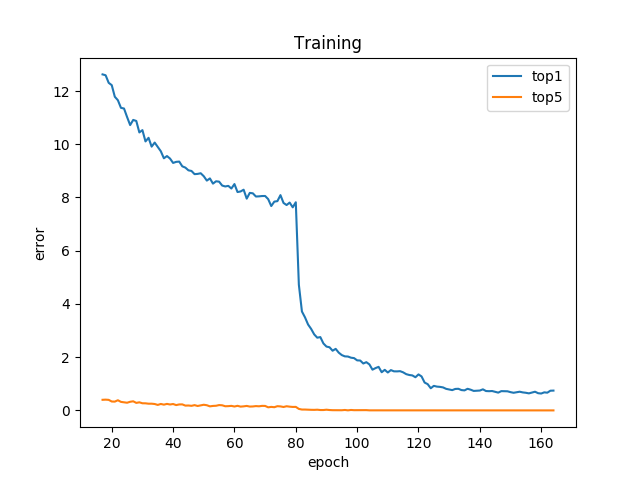
\includegraphics[width=1.0\textwidth]{\path/ResNet-Cifar10-Train.png} 
 \caption{Top-1 e Top-5 training accuracy di ResNet sul dataset CIFAR10}
 \label{fig:res-train}
\end{figure}

\begin{figure}[h!]
 \centering
 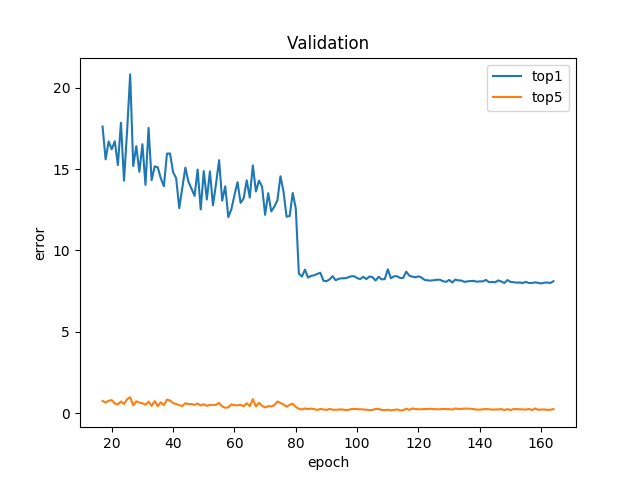
\includegraphics[width=1.0\textwidth]{\path/ResNet-Cifar10-Val.png} 
 \caption{Top-1 e Top-5 validation accuracy di ResNet sul dataset CIFAR10}
 \label{fig:res-val}
\end{figure}

\section{LeNet vs ResNet: confronto}
Nel Capitolo \ref{Capitolo4} si è addestrato uno dei primi modelli di CNN sullo stesso dataset, CIFAR10. La superiorità di ResNet è evidente, raggiunge un'accuratezza di circa il 92-93\% laddove LeNet arrivava appena ad un 73\%. \\
Questo è dovuto a diversi elementi, ma sicuramente è una riprova del fatto che aumentando il numero di layer di convoluzione si aumenta la ricchezza della rappresentazione delle features delle immagini in ingresso e di conseguenza aumenta la capacità della rete di astrarre e "comprendere" molto meglio le informazioni nelle immagini. \\
Ogni anno le architetture delle reti subiscono variazioni e vengono introdotte novità dirompenti che generano nuove riflessioni che spingono quest'ambito di ricerca in avanti ad una velocità tale da mantenere il passo con l'industria delle GPU di cui hanno bisogno per essere  realizzate. 



 
% Chapter Template

\chapter{Conclusioni} % Main c




% Chapter Template

\chapter{Conclusioni} % Main c





%----------------------------------------------------------------------------------------
%	THESIS CONTENT - APPENDICES
%----------------------------------------------------------------------------------------

\appendix % Cue to tell LaTeX that the following "chapters" are Appendices

% Include the appendices of the thesis as separate files from the Appendices folder
% Uncomment the lines as you write the Appendices

%
% Appendix A

\chapter{MLP: Codice addizionale} % Main appendix title

\label{AppendixA} % Change X to a consecutive letter; for referencing this appendix elsewhere, use \ref{AppendixX}

\section{Classi in Lua}
In Lua manca il costrutto delle classi. Si può tuttavia crearle utilizzando tables e meta-tables. Per realizzare il multi-layer perceptron si è utilizzato una piccola libreria, di seguito riportata. 

\begin{lstlisting}[language={[5.2]Lua}]
-- class.lua
-- Compatible with Lua 5.1 (not 5.0).
function class(base, init)
   local c = {} -- a new class instance
   if not init and type(base) == 'function' then
      init = base
      base = nil
   elseif type(base) == 'table' then
      -- our new class is a shallow copy of the base class!
      for i,v in pairs(base) do
         c[i] = v
      end
      c._base = base
   end
   -- the class will be the metatable for all its objects,
   -- and they will look up their methods in it.
   c.__index = c

   -- expose a constructor which can be called by <classname>(<args>)
   local mt = {}
   mt.__call = function(class_tbl, ...)
      local obj = {}
      setmetatable(obj,c)
      if init then
         init(obj,...)
      else
         -- make sure that any stuff from the base class is initialized!
         if base and base.init then
            base.init(obj, ...)
         end
      end
      return obj
   end
   c.init = init
   c.is_a = function(self, klass)
      local m = getmetatable(self)
      while m do
         if m == klass then return true end
         m = m._base
      end
      return false
   end
   setmetatable(c, mt)
   return c
end
\end{lstlisting}
\section{La classe Neural\_Network}
Nel capitolo \ref{Capitolo2} si sono mostrati i vari snippet di codice man mano che si introducevano i concetti teorici che stanno alla base di questa implementazione. Di seguito è presentata l'intera classe \texttt{Neural\_Network} :

\begin{lstlisting}[language={[5.2]Lua}]
--creating class NN in Lua, using a nice class utility
class = require 'class'

Neural_Network = class('Neural_Network')

--init NN
function Neural_Network:__init(inputs, hiddens, outputs)
      self.inputLayerSize = inputs
      self.hiddenLayerSize = hiddens
      self.outputLayerSize = outputs
      self.W1 = th.randn(net.inputLayerSize, self.hiddenLayerSize)
      self.W2 = th.randn(net.hiddenLayerSize, self.outputLayerSize)
end

--define a forward method
function Neural_Network:forward(X)
   --Propagate inputs though network
   self.z2 = th.mm(X, self.W1)
   self.a2 = th.sigmoid(self.z2)
   self.z3 = th.mm(self.a2, self.W2)
   yHat = th.sigmoid(self.z3)
   return yHat
end

function Neural_Network:d_Sigmoid(z)
   --derivative of the sigmoid function
   return th.exp(-z):cdiv( (th.pow( (1+th.exp(-z)),2) ) )
end

function Neural_Network:costFunction(X, y)
   --Compute the cost for given X,y, use weights already stored in class
   self.yHat = self:forward(X)
   --NB torch.sum() isn't equivalent to python sum() built-in method
   --However, for 2D arrays whose one dimension is 1, it won't make any difference
   J = 0.5 * th.sum(th.pow((y-yHat),2))
   return J
end

function Neural_Network:d_CostFunction(X, y)
   --Compute derivative wrt to W1 and W2 for a given X and y
   self.yHat = self:forward(X)
   delta3 = th.cmul(-(y-self.yHat), self:d_Sigmoid(self.z3))
   dJdW2 = th.mm(self.a2:t(), delta3)

   delta2 = th.mm(delta3, self.W2:t()):cmul(self:d_Sigmoid(self.z2))
   dJdW1 = th.mm(X:t(), delta2)

   return dJdW1, dJdW2
end

\end{lstlisting}

\section{Metodi getter e setter}
Nella sottosezione \ref{sec:gradcheck} del capitolo \ref{Capitolo2} si è dimostrato come calcolare numericamente il gradiente. Si è fatto cenno ai \emph{getter e setter} per ottenere dei \emph{flattened gradients}, ovvero "srotolare" i tensori dei gradienti in vettori monodimensionali. I metodi, qui mostrati, necessitano di una comprensione dei comandi di Torch. Data la maggiore popolarità di Python \emph{Numpy}, nel caso il lettore fosse più familiare con quest'ultimo, nell'appendice \ref{AppendixB} è mostrata anche una tabella di equivalenza dei metodi fra i due. 
\begin{lstlisting}[language={[5.2]Lua}]
--Helper Functions for interacting with other classes:
function Neural_Network:getParams()
   --Get W1 and W2 unrolled into a vector
   params = th.cat((self.W1:view(self.W1:nElement())), (self.W2:view(self.W2:nElement())))
   return params
end

function Neural_Network:setParams(params)
   --Set W1 and W2 using single paramater vector.
   W1_start = 1 --index starts at 1 in Lua
   W1_end = self.hiddenLayerSize * self.inputLayerSize
   self.W1 = th.reshape(params[{ {W1_start, W1_end} }], self.inputLayerSize, self.hiddenLayerSize)
   W2_end = W1_end + self.hiddenLayerSize*self.outputLayerSize
   self.W2 = th.reshape(params[{ {W1_end+1, W2_end} }], self.hiddenLayerSize, self.outputLayerSize)
end

--this is like the getParameters(): method in the NN module of torch, i.e. compute the gradients and returns a flattened grads array
function Neural_Network:computeGradients(X, y)
   dJdW1, dJdW2 = self:d_CostFunction(X, y)
   return th.cat((dJdW1:view(dJdW1:nElement())), (dJdW2:view(dJdW2:nElement())))
end
\end{lstlisting}

% Appendix Template

\chapter{Il framework Torch} % Main appendix title
\label{AppendixB} % Change X to a consecutive letter; for referencing this appendix elsewhere, use \ref{AppendixX}
\def \path {Appendices/}
\section{Introduzione}
Torch\parencite{WTorch} è un framework per il calcolo numerico versatile che estende il linguaggio Lua. L'obiettivo è quello di fornire un ambiente flessibile per il progetto e addestramento di sistemi di machine learning anche su larga scala.\\
La flessibilità è ottenuta grazie a Lua stesso, un linguaggio di scripting estremamente leggero e efficiente. Le prestazioni sono garantite da backend compilati ed ottimizzati (C,C++,CUDA,OpenMP/SSE) per le routine di calcolo numerico di basso livello.
\\
\\
Gli obiettivi degli autori erano: (1) facilità di sviluppo di algoritmi numerici; (2) facilità di
estensione, incluso il supporto ad altre librerie; (3) la velocità.\\
Gli obiettivi (2) e (3) sono stati soddisfatti tramite l'utilizzo di Lua poiché un linguaggio interpretato risulta conveniente per il testing rapido in modo interattivo; garantisce facilità di sviluppo e, grazie alle ottime C-API, unisce in modo eterogeneo le varie librerie,
nascondendole sotto un'unica struttura di linguaggio di scripting.  Infine, essendo ossessionati dalla velocità, è stato scelto Lua poiché è un veloce linguaggio di scripting e può inoltre contare su un efficiente compilatore JIT.
Inoltre, Lua ha il grosso vantaggio di essere stato progettato per essere facilmente inserito nelle applicazioni scritte in C e consente quindi di “wrappare” le sottostanti implementazioni in C/C++ in maniera banale. Il binding C per il Lua è tra i più semplici e dona quindi grande estensibilità al progetto Torch. 
\\
\\
Torch è un framework auto-contenuto e estremamente portabile su ogni piattaforma: iOS, Android, FPGA, processori DSP ecc. Gli scrpt che vengono scritti per Torch riescono ad essere eseguiti su queste piattaforme senza nessuna modifica.
\\
Per soddisfare il requisito (1) hanno invece ideato un oggetto chiamato \texttt{'Tensor'}, il quale altro non è che una “vista” geometrica di una particolare area di memoria, e permette una efficiente e semplice 
gestione di vettori a N dimensioni, tensori appunto.\\
L’oggetto Tensor fornisce anche un’efficiente gestione della memoria: ogni operazione fatta su di esso non alloca nuova memoria, ma trasforma il tensore esistente o ritorna un nuovo tensore che referenzia la stessa area di memoria.
Torch fornisce un ricco set di routine di calcolo numerico: le comuni routine di Matlab, algebra lineare, convoluzioni, FFT, ecc. Ci sono molti package per diversi ambiti: Machine Learning, Visione Artificiale, Image \& Video Processing, Speech Recognition, ecc.\\
\\
I package più importanti per il machine learning sono: 
\begin{itemize}
\item \textbf{nn}: Neural Network, fornisce ogni sorta di modulo per la costruzione di reti neurali, reti neural profonde (deep), regressione lineare, MLP, autoencoders ecc. È il package utilizzato nel progetto. Per topologie di rete bleeding-edge si suggerisce il package \textbf{'nnx'}; 
\item  \textbf{optim}: package per l'ottimizzazione della discesa del gradiente  Fondamentale per avere buone performance nel training della rete; 
\item \textbf{unsup}: è un toolbox per l'apprendimento non supervisionato; 

\item \textbf{Image}: contiene tutte le funzioni atte all'image processing; 

\item \textbf{cunn}: package per utilizzare le reti neurali sfruttando la potenza di calcolo parallelo delle GPU, mediante l'architettura CUDA. 
\end{itemize}
L'architettura del framework è raffigurata in figura \ref{fig:torch}.\\

\begin{figure}[h!]
 \centering
 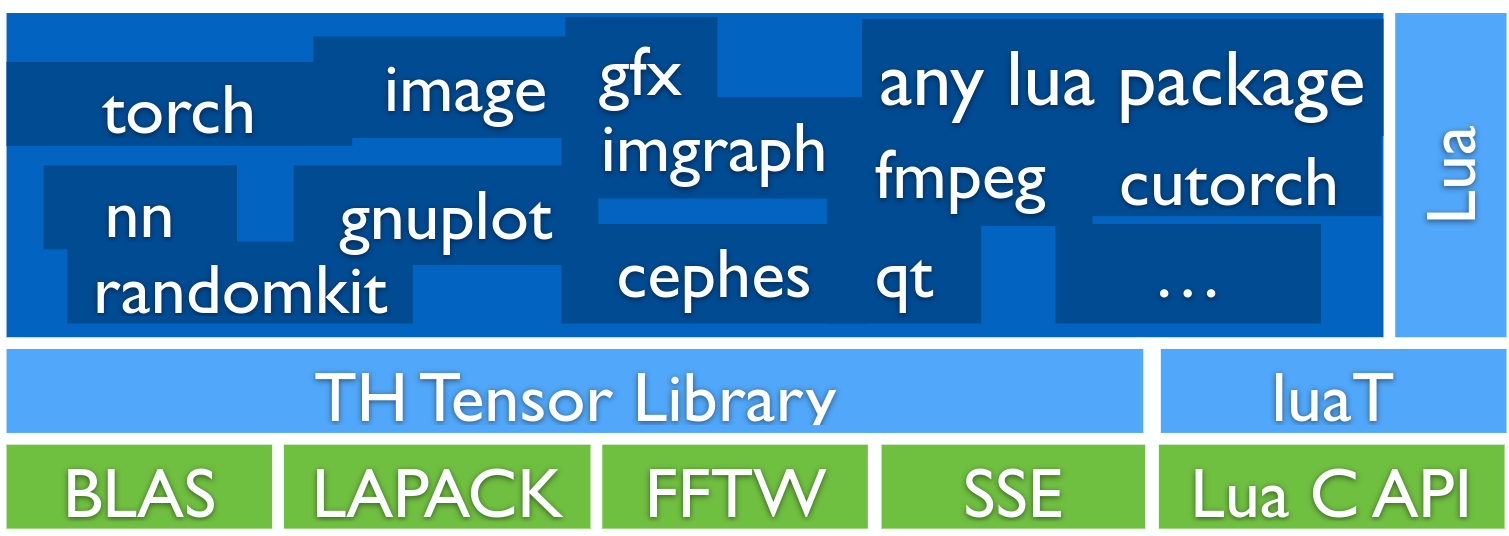
\includegraphics[width=1.0\textwidth]{\path/torch.png} 
 \caption{Architettura del framework Torch}
 \label{fig:torch}
\end{figure}
\\
Torch è adottato da una fiorente comunità attiva di ricercatori in diverse università e importanti centri di ricerca come quelli di IBM; il dipartimento di IA di Facebook (FAIR); Google DeepMind prima di passare a TensorFlow nel 2016.

\section{Utilizzo base per reti neurali}
Costruire modelli di reti neurali è una procedura rapida con Torch, ecco alcuni esempi: 
\begin{lstlisting}[language={[5.2]Lua}]
------------------------------------------------------------
-- simple linear model: logistic regression
------------------------------------------------------------
model:add(nn.Reshape(3*32*32))
model:add(nn.Linear(3*32*32,#classes))

------------------------------------------------------------
-- classic 2-layer fully-connected MLP
------------------------------------------------------------
model:add(nn.Reshape(3*32*32))
model:add(nn.Linear(3*32*32, 1*32*32))
model:add(nn.ReLU())
model:add(nn.Linear(1*32*32, #classes))

------------------------------------------------------------
-- convolutional layer
------------------------------------------------------------
--hyper-parameters
nfeats = 3 --3D input volume
nstates = {16, 64, 128} --output at each level
filtsize = 5 --filter size or kernel 
poolsize = 2

--Here's only the first stage. 
--The others look the same except for the nstates you're gonna use

-- filter bank -> squashing -> max pooling
model:add(nn.SpatialConvolutionMM(nfeats, nstates[1], filtsize, filtsize))
model:add(nn.ReLU())
model:add(nn.SpatialMaxPooling(poolsize, poolsize, poolsize, poolsize))
\end{lstlisting}
\subsection{Supporto CUDA}
CUDA (Compute Unified Device Architecture) è l'architettura di elaborazione in parallelo di NVIDIA che permette netti aumenti delle prestazioni di computing grazie allo sfruttamento della potenza di calcolo delle GPU per operazioni “general purpose”.\\
Torch offre un package chiamato \texttt{'cunn'} per usufruire di CUDA. Il package è basato su un tensore chiamato \texttt{'torch.CudaTensor()'} che altro non è che un normale Tensor che risiede ed utilizza la memoria della DRAM della GPU; tutte le operazioni definite per l'oggetto Tensor sono definite normalmente anche per il CudaTensor, il quale astrae completamente dall'utilizzo della GPU, offrendo un'interfaccia semplice e permettendo di sfruttare gli stessi script che si usano per l'elaborazione CPU. L'unica modifica da apportare, quindi, è cambiare il tipo di tensore. 
\begin{lstlisting}[language={[5.2]Lua}]
tf = torch.FloatTensor(4,100,100) -- CPU's DRAM
tc = tf:cuda() -- GPU's DRAM 
tc:mul() -- run on GPU
res = tc:float() -- res is instantiated on CPU's DRAM

--similarly, after we've built our model
--we can move it to the GPU by doing
model:cuda()
--we also need to compute our loss on GPU
criterion:cuda()

--now we're set, we can train our model on the GPU 
--just by following the standard training procedure seen in (Capitolo 4)
\end{lstlisting}


\section{ResNet}
Una rappresentazione testuale del modello a 18 strati di Residual Network. 

\begin{lstlisting}[language={[5.2]Lua}]
nn.Sequential {
  [input -> (1) -> (2) -> (3) -> (4) -> (5) -> (6) -> (7) -> (8) -> (9) -> output]
  (1): cudnn.SpatialConvolution(3 -> 16, 3x3, 1,1, 1,1) without bias
  (2): nn.SpatialBatchNormalization (4D) (16)
  (3): cudnn.ReLU
  (4): nn.Sequential {
    [input -> (1) -> (2) -> (3) -> output]
    (1): nn.Sequential {
      [input -> (1) -> (2) -> (3) -> output]
      (1): nn.ConcatTable {
        input
          |`-> (1): nn.Sequential {
          |      [input -> (1) -> (2) -> (3) -> (4) -> (5) -> output]
          |      (1): cudnn.SpatialConvolution(16 -> 16, 3x3, 1,1, 1,1) without bias
          |      (2): nn.SpatialBatchNormalization (4D) (16)
          |      (3): cudnn.ReLU
          |      (4): cudnn.SpatialConvolution(16 -> 16, 3x3, 1,1, 1,1) without bias
          |      (5): nn.SpatialBatchNormalization (4D) (16)
          |    }
           `-> (2): nn.Identity
           ... -> output
      }
      (2): nn.CAddTable
      (3): cudnn.ReLU
    }
    (2): nn.Sequential {
      [input -> (1) -> (2) -> (3) -> output]
      (1): nn.ConcatTable {
        input
          |`-> (1): nn.Sequential {
          |      [input -> (1) -> (2) -> (3) -> (4) -> (5) -> output]
          |      (1): cudnn.SpatialConvolution(16 -> 16, 3x3, 1,1, 1,1) without bias
          |      (2): nn.SpatialBatchNormalization (4D) (16)
          |      (3): cudnn.ReLU
          |      (4): cudnn.SpatialConvolution(16 -> 16, 3x3, 1,1, 1,1) without bias
          |      (5): nn.SpatialBatchNormalization (4D) (16)
          |    }
           `-> (2): nn.Identity
           ... -> output
      }
      (2): nn.CAddTable
      (3): cudnn.ReLU
    }
    (3): nn.Sequential {
      [input -> (1) -> (2) -> (3) -> output]
      (1): nn.ConcatTable {
        input
          |`-> (1): nn.Sequential {
          |      [input -> (1) -> (2) -> (3) -> (4) -> (5) -> output]
          |      (1): cudnn.SpatialConvolution(16 -> 16, 3x3, 1,1, 1,1) without bias
          |      (2): nn.SpatialBatchNormalization (4D) (16)
          |      (3): cudnn.ReLU
          |      (4): cudnn.SpatialConvolution(16 -> 16, 3x3, 1,1, 1,1) without bias
          |      (5): nn.SpatialBatchNormalization (4D) (16)
          |    }
           `-> (2): nn.Identity
           ... -> output
      }
      (2): nn.CAddTable
      (3): cudnn.ReLU
    }
  }
  (5): nn.Sequential {
    [input -> (1) -> (2) -> (3) -> output]
    (1): nn.Sequential {
      [input -> (1) -> (2) -> (3) -> output]
      (1): nn.ConcatTable {
        input
          |`-> (1): nn.Sequential {
          |      [input -> (1) -> (2) -> (3) -> (4) -> (5) -> output]
          |      (1): cudnn.SpatialConvolution(16 -> 32, 3x3, 2,2, 1,1) without bias
          |      (2): nn.SpatialBatchNormalization (4D) (32)
          |      (3): cudnn.ReLU
          |      (4): cudnn.SpatialConvolution(32 -> 32, 3x3, 1,1, 1,1) without bias
          |      (5): nn.SpatialBatchNormalization (4D) (32)
          |    }
           `-> (2): nn.Sequential {
                 [input -> (1) -> (2) -> output]
                 (1): nn.SpatialAveragePooling(1x1, 2,2)
                 (2): nn.Concat {
                   input
                     |`-> (1): nn.Identity
                      `-> (2): nn.MulConstant
                      ... -> output
                 }
               }
           ... -> output
      }
      (2): nn.CAddTable
      (3): cudnn.ReLU
    }
    (2): nn.Sequential {
      [input -> (1) -> (2) -> (3) -> output]
      (1): nn.ConcatTable {
        input
          |`-> (1): nn.Sequential {
          |      [input -> (1) -> (2) -> (3) -> (4) -> (5) -> output]
          |      (1): cudnn.SpatialConvolution(32 -> 32, 3x3, 1,1, 1,1) without bias
          |      (2): nn.SpatialBatchNormalization (4D) (32)
          |      (3): cudnn.ReLU
          |      (4): cudnn.SpatialConvolution(32 -> 32, 3x3, 1,1, 1,1) without bias
          |      (5): nn.SpatialBatchNormalization (4D) (32)
          |    }
           `-> (2): nn.Identity
           ... -> output
      }
      (2): nn.CAddTable
      (3): cudnn.ReLU
    }
    (3): nn.Sequential {
      [input -> (1) -> (2) -> (3) -> output]
      (1): nn.ConcatTable {
        input
          |`-> (1): nn.Sequential {
          |      [input -> (1) -> (2) -> (3) -> (4) -> (5) -> output]
          |      (1): cudnn.SpatialConvolution(32 -> 32, 3x3, 1,1, 1,1) without bias
          |      (2): nn.SpatialBatchNormalization (4D) (32)
          |      (3): cudnn.ReLU
          |      (4): cudnn.SpatialConvolution(32 -> 32, 3x3, 1,1, 1,1) without bias
          |      (5): nn.SpatialBatchNormalization (4D) (32)
          |    }
           `-> (2): nn.Identity
           ... -> output
      }
      (2): nn.CAddTable
      (3): cudnn.ReLU
    }
  }
  (6): nn.Sequential {
    [input -> (1) -> (2) -> (3) -> output]
    (1): nn.Sequential {
      [input -> (1) -> (2) -> (3) -> output]
      (1): nn.ConcatTable {
        input
          |`-> (1): nn.Sequential {
          |      [input -> (1) -> (2) -> (3) -> (4) -> (5) -> output]
          |      (1): cudnn.SpatialConvolution(32 -> 64, 3x3, 2,2, 1,1) without bias
          |      (2): nn.SpatialBatchNormalization (4D) (64)
          |      (3): cudnn.ReLU
          |      (4): cudnn.SpatialConvolution(64 -> 64, 3x3, 1,1, 1,1) without bias
          |      (5): nn.SpatialBatchNormalization (4D) (64)
          |    }
           `-> (2): nn.Sequential {
                 [input -> (1) -> (2) -> output]
                 (1): nn.SpatialAveragePooling(1x1, 2,2)
                 (2): nn.Concat {
                   input
                     |`-> (1): nn.Identity
                      `-> (2): nn.MulConstant
                      ... -> output
                 }
               }
           ... -> output
      }
      (2): nn.CAddTable
      (3): cudnn.ReLU
    }
    (2): nn.Sequential {
      [input -> (1) -> (2) -> (3) -> output]
      (1): nn.ConcatTable {
        input
          |`-> (1): nn.Sequential {
          |      [input -> (1) -> (2) -> (3) -> (4) -> (5) -> output]
          |      (1): cudnn.SpatialConvolution(64 -> 64, 3x3, 1,1, 1,1) without bias
          |      (2): nn.SpatialBatchNormalization (4D) (64)
          |      (3): cudnn.ReLU
          |      (4): cudnn.SpatialConvolution(64 -> 64, 3x3, 1,1, 1,1) without bias
          |      (5): nn.SpatialBatchNormalization (4D) (64)
          |    }
           `-> (2): nn.Identity
           ... -> output
      }
      (2): nn.CAddTable
      (3): cudnn.ReLU
    }
    (3): nn.Sequential {
      [input -> (1) -> (2) -> (3) -> output]
      (1): nn.ConcatTable {
        input
          |`-> (1): nn.Sequential {
          |      [input -> (1) -> (2) -> (3) -> (4) -> (5) -> output]
          |      (1): cudnn.SpatialConvolution(64 -> 64, 3x3, 1,1, 1,1) without bias
          |      (2): nn.SpatialBatchNormalization (4D) (64)
          |      (3): cudnn.ReLU
          |      (4): cudnn.SpatialConvolution(64 -> 64, 3x3, 1,1, 1,1) without bias
          |      (5): nn.SpatialBatchNormalization (4D) (64)
          |    }
           `-> (2): nn.Identity
           ... -> output
      }
      (2): nn.CAddTable
      (3): cudnn.ReLU
    }
  }
  (7): cudnn.SpatialAveragePooling(8x8, 1,1)
  (8): nn.View(64)
  (9): nn.Linear(64 -> 10)
}

\end{lstlisting}
%\include{Appendices/AppendixC}

%----------------------------------------------------------------------------------------
%	BIBLIOGRAPHY
%----------------------------------------------------------------------------------------

\printbibliography[heading=bibintoc]

%----------------------------------------------------------------------------------------

\end{document}  
